%%%%%%%%%%%%%%%%%%%%%%%%%%%%%%%%%%%%%%%%%%%%%%%%%%
% 既存研究サーベイ（網羅版）
% 事前学習VLM検出器のドメイン増加型継続学習
% MPRG Work Document Template ベース
%%%%%%%%%%%%%%%%%%%%%%%%%%%%%%%%%%%%%%%%%%%%%%%%%%
\RequirePackage[l2tabu, orthodox]{nag}
\documentclass[11pt, a4j]{jarticle}
\usepackage{mprg}
\usepackage{datetime}
\usepackage{ascmac}

\begin{document}

\title{事前学習済み Vision-Language Model 検出器の\\
ドメイン増加型継続学習に関する既存研究サーベイ（網羅版）}
\author{TP26801 今井　孝洋}
\date{2026年6月22日}
\maketitle
\pagestyle{fancy}

%==================================================================
\section{はじめに：研究設定と課題}
本稿は，事前学習済み Vision-Language Model（VLM）検出器
（MM-Grounding DINO~\cite{mmgdino}）を対象とした
ドメインが増加する物体検出の継続学習（domain-incremental continual learning; DIL）について，
関連する既存研究を網羅的かつ専門的に整理する自分用のリファレンスである．
本設定は次の三つの要件を同時に満たす必要がある．
\begin{itemize}
  \item (A) 新ドメインへの適応：事前学習に乏しい専門ドメインへ検出性能を引き上げる．
  \item (B) 過去ドメインの忘却抑制：逐次学習で過去に学習したドメインを忘れない．
  \item (C) ゼロショット汎化の保持（ZCOCO）：事前学習由来の汎用検出能力（COCO 検出）を保持する．
\end{itemize}

課題(A)の深刻さは図~\ref{fig:gap}に示される．Grounding DINO は一般的な ODinW-13 では
ゼロショットで 49.2~mAP に達するが，VLM 事前学習に乏しい概念を含む Roboflow100-VL~\cite{rf100vl}
ではゼロショット平均 16~mAP，医療ドメインでは 2\%未満まで低下する．
課題(B)(C)は，新ドメインへ素朴に逐次 fine-tune すると，共有検出経路が上書きされて
過去ドメインと COCO の双方を破滅的に忘却することに対応する．
これら(A)(B)(C)を同時に満たす「事前学習 VLM 検出器のドメイン増加型継続学習」は未開拓である．
本研究の提案手法は，本体を凍結し各ドメインを低ランク適応（LoRA）で学習しつつ，
更新部分空間を過去タスクおよび COCO（task-0）の勾配空間と直交化する InfLoRA 型の枠組みであり，
最も近い競合は ZiRa~\cite{zira} と DitHub~\cite{dithub} である．

\begin{figure}[tb]
\centering
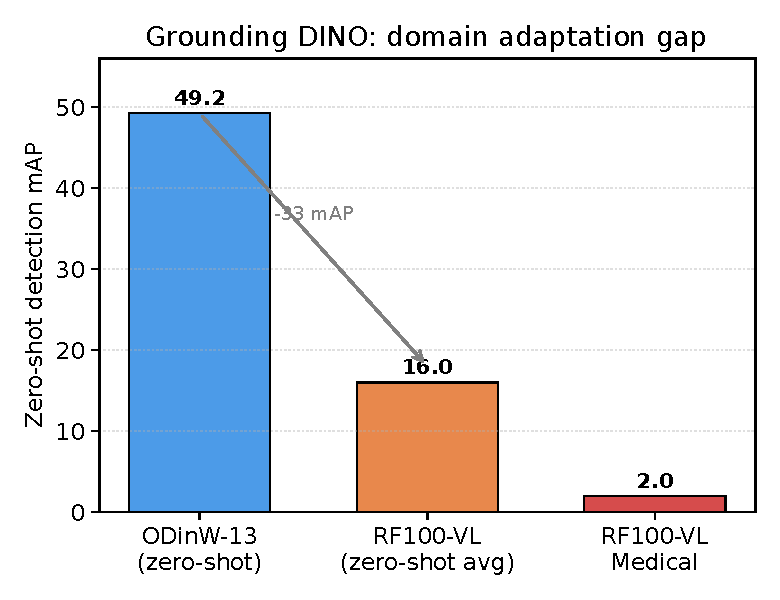
\includegraphics[width=0.6\linewidth]{figs/fig2_adaptation_gap.pdf}
\caption{事前学習 VLM 検出器の適応ギャップ（課題A）．Grounding DINO のゼロショット検出 mAP は，
一般ドメイン（ODinW-13）から専門ドメイン（RF100-VL）で大きく低下する~\cite{rf100vl}．}
\label{fig:gap}
\end{figure}

本稿の構成は次の通りである．
第\ref{sec:ovd}節でオープン語彙検出と継続物体検出の地形図を整理し，
第\ref{sec:theory}節で継続学習の基礎と忘却の理論を，
第\ref{sec:lora}節で提案手法の基盤となる LoRA/PEFT ベース継続学習を深掘りする．
第\ref{sec:toolbox}節で忘却機序分析（C2）に転用できる方法論を整理し，
第\ref{sec:vlmcl}節で直接競合となる VLM/OVD 継続学習とゼロショット保持の手法群を扱う．
第\ref{sec:novelty}節で本研究の位置づけと新規性を述べ，第\ref{sec:conclusion}節でまとめる．

%==================================================================
\section{オープン語彙検出と継続物体検出の地形図}
\label{sec:ovd}
\section{継続物体検出とオープン語彙検出の地形図}
\label{sec:detection_ovd}

本章では，本研究の基盤検出器であるMM-Grounding DINO \cite{mmgdino} を中心に，オープン語彙検出（OVD）の系譜，継続学習と物体検出の交差点，および評価基盤と適応ギャップの三領域を整理する．特に，二段検出器で観測された「忘却は分類側に局在し，回帰側は頑健」という知見 \cite{nsgp,redistill} が，クエリベースかつ視覚-言語対照ヘッドを持つMM-Grounding DINOへ転移するか否かを，本研究で検証すべき仮説として位置づける．


\subsection{オープン語彙検出の定式化と系譜}
\label{subsec:ovd_lineage}

\paragraph{問題設定と動機．}
従来の閉集合検出器は，学習時に固定したカテゴリ集合 $\mathcal{C}_{\mathrm{base}}$ のみを検出できる．これに対しオープン語彙検出は，推論時に任意のテキスト語彙 $\mathcal{C}_{\mathrm{test}}$（$\mathcal{C}_{\mathrm{base}} \subseteq \mathcal{C}_{\mathrm{test}}$ とは限らない）を入力として与え，学習時に箱アノテーションを見ていない新規カテゴリ（novel）も検出することを目指す．動機は，物体検出の語彙を分類器の重み行列から切り離し，視覚-言語事前学習で得た意味空間に接続することで，スケーラブルな汎化を得る点にある．

\paragraph{中核アイデアと系譜．}
OVDのサーベイ \cite{ovdsurvey} に従うと，主要な技術系譜は次のように整理できる．
\begin{enumerate}
\item 視覚-意味マッピング：領域特徴をCLIP \cite{clip} などの埋め込み空間へ射影し，クラス名のテキスト埋め込みとの類似度で分類する（RegionCLIP \cite{regionclip}）．
\item 領域認識のグラウンディング学習：検出を句グラウンディングとして再定式化し，画像-テキスト対の大規模コーパスで領域-語の対応を学習する（GLIP \cite{glip}，Grounding DINO \cite{groundingdino}）．
\item 擬似ラベルと弱教師：画像分類データやキャプションから擬似的な箱ラベルを生成して語彙を拡張する（Detic \cite{detic}）．
\item 蒸留と転移：CLIPの画像-テキスト整合性を検出器へ蒸留する，あるいはViTベースの検出ヘッドを軽量に転移する（OWL-ViT \cite{owlvit}，YOLO-World \cite{yoloworld}）．
\end{enumerate}
これらは相互排他的でなく，現代の基盤検出器はグラウンディング学習と擬似ラベル，蒸留を組み合わせる．

\paragraph{定式化．}
OVDの共通骨格は，領域特徴 $\mathbf{v} \in \mathbb{R}^{d}$ とテキスト埋め込み $\{\mathbf{t}_{c}\}_{c \in \mathcal{C}_{\mathrm{test}}}$ の整合度に基づく分類である．カテゴリ $c$ の予測スコアは内積（対照ロジット）
\begin{equation}
s_{c} = \frac{\langle \mathbf{v},\, \mathbf{t}_{c}\rangle}{\tau},\qquad
p_{c} = \sigma\!\left(s_{c}\right),
\label{eq:ovd_logit}
\end{equation}
で与えられる．ここで $\tau$ は温度，$\sigma$ はシグモイド（または語彙上のソフトマックス）である．閉集合検出器が学習可能な分類器重み $\mathbf{w}_{c}$ を用いるのに対し，OVDでは $\mathbf{t}_{c}$ をテキストエンコーダの出力で置換することで，語彙を推論時に差し替え可能にする点が本質である．

\paragraph{評価設定．}
OVDの代表的評価はOV-COCO／OV-LVIS（base/novelの分割，novelのAP）と，多様なドメインを横断するODinW（Object Detection in the Wild）である．ODinW-13上でGrounding DINOはゼロショットで49.2 mAPを達成する \cite{rf100vl}．

\paragraph{長所と短所．}
長所は語彙の柔軟性とゼロショット汎化である．短所は，事前学習分布から離れた専門ドメイン（医療，顕微鏡，電磁波など）で性能が急落すること（後述 \ref{subsec:rf100}），およびテキスト依存ゆえにクラス名の言語的曖昧性に敏感なことである．

\paragraph{本研究への含意．}
本研究の基盤MM-Grounding DINOはグラウンディング学習系に属し，式 \eqref{eq:ovd_logit} の対照ロジットを検出ヘッドに持つ．ドメイン増加型継続学習において保護すべき資産は，閉集合分類器の重みではなく，テキスト埋め込み空間と領域-語整合の汎化能力（ZCOCO）である点が，閉集合の継続物体検出とは本質的に異なる．


\subsection{基盤検出器MM-Grounding DINOの構造}
\label{subsec:mmgdino}

\paragraph{位置づけと動機．}
MM-Grounding DINO \cite{mmgdino} は，Grounding DINO \cite{groundingdino} をオープンソースの大規模データで再実装・拡張した基盤検出器であり，公開された学習レシピと多ドメイン評価を備える．本研究はこれを継続学習の対象VLMとして採用する．

\paragraph{構造（モジュール分解）．}
MM-Grounding DINOは次の要素から構成される．
\begin{enumerate}
\item 画像バックボーン：Swin Transformer によるマルチスケール視覚特徴抽出．
\item テキストエンコーダ：BERT によるクラス名・プロンプトの埋め込み．
\item 特徴強調器（feature enhancer）：変形可能自己注意（画像側）とテキスト自己注意，および双方向のクロスモーダル注意により，視覚特徴とテキスト特徴を相互に条件づける．
\item 言語誘導クエリ選択（language-guided query selection）：テキストとの類似度が高い画像トークンをデコーダのクエリ初期化に選ぶ機構．
\item クロスモダリティデコーダ：DINO型のクエリを画像・テキスト双方の注意で更新する．
\item 対照ヘッド：各クエリの出力と各テキストトークン埋め込みの内積で，クエリ-語の整合ロジットを算出する（式 \eqref{eq:ovd_logit} に対応）．箱回帰は別ブランチで座標を予測する．
\end{enumerate}

\paragraph{定式化．}
$N$ 個のデコーダ出力クエリ $\{\mathbf{q}_{i}\}_{i=1}^{N}$ と $L$ 個のテキストトークン埋め込み $\{\mathbf{t}_{j}\}_{j=1}^{L}$ に対し，整合ロジット行列 $\mathbf{S} \in \mathbb{R}^{N \times L}$ は
\begin{equation}
S_{ij} = \langle \mathbf{q}_{i},\, \mathbf{t}_{j}\rangle,
\label{eq:mmg_logit}
\end{equation}
で与えられ，カテゴリ $c$ の語が占めるトークン集合 $\mathcal{T}_{c}$ 上の集約（最大または平均）でクエリ $i$ のクラス $c$ スコアを得る．分類損失は焦点損失型の対照損失，箱は $L_{1}$ とGIoUの和で，二部マッチングにより教師と対応づける．

\paragraph{テキストトークン長の制約．}
対照ヘッドは全カテゴリ名を結合したテキスト系列に依存するため，トークン長上限（既定 \texttt{max\_text\_len}$=256$）を超える多クラスドメインでは失敗する．本研究ではconfigで $512$ 等へ拡張する（顕微鏡や実世界の多クラス設定）．

\paragraph{長所と短所．}
長所は，分類器が学習可能重みでなくテキスト埋め込みに置換されているため，語彙差し替えとゼロショットが自然なこと，公開レシピで再現性が高いことである．短所は，モデルが大きく，専門ドメインへの適応にはファインチューニングが必要で，その際に事前学習汎化（ZCOCO）と過去ドメインの忘却が生じる点である．

\paragraph{本研究への含意．}
継続学習の介入対象は，バックボーン・特徴強調器・デコーダ・対照ヘッドのいずれにも置きうる．二段検出器の知見 \cite{nsgp,redistill} を踏まえると，忘却がクエリ-語整合（対照ヘッド・テキスト側）に局在するのか，箱回帰ブランチが頑健なのかを，モジュール局在化分析で確認することが第一の問いとなる（\ref{subsec:nsgp} 参照）．


\subsection{CL-DETR：DETR系継続学習と汎用蒸留・リプレイの限界}
\label{subsec:cldetr}

\paragraph{問題設定と動機．}
増分物体検出（IOD）は，段階ごとに新カテゴリのアノテーションを与えて検出器を更新する設定であり，破滅的忘却を被る \cite{cldetr}．従来は知識蒸留（KD）と模範例リプレイ（ER）で対処してきたが，CL-DETR \cite{cldetr} はこれらを Deformable DETR や UP-DETR などの最新Transformer検出器へ素朴に適用しても十分に機能しないことを指摘した．

\paragraph{中核アイデア．}
CL-DETRは二点の検出器固有適応を導入する．第一に検出器知識蒸留（DKD）で，旧モデルの予測のうち最も情報量が高く信頼できるものに絞って蒸留し，冗長な背景予測を無視し，現タスクの正解ラベルと両立させる．第二に較正済みリプレイで，観測したカテゴリ分布を保つよう模範例をサンプルする．

\paragraph{手順と評価．}
COCO 2017上のIOD設定（例：$40+40$ や $70+10$ のカテゴリ分割）で評価し，当時のSOTAを達成した \cite{cldetr}．

\paragraph{長所と短所．}
長所は，DETR系に蒸留・リプレイを有効化したこと，および「汎用CL手法をそのまま検出器へ適用すると失敗する」ことを明確化した点である．短所は，設定がクラス増分中心であり，純粋なドメイン増分やOVDのゼロショット保持を扱わないこと，模範例保持が前提でプライバシ・記憶制約と相反しうることである．なお，これは2023年時点の知見であり現行SOTAとして引用するものではない．

\paragraph{本研究への含意．}
MM-Grounding DINOもDETR系クエリ検出器であるため，汎用KD/ERの素朴適用が不十分という教訓は本研究に直接適用される．対照ヘッドを持つVLM検出器では，蒸留対象を「旧モデルの整合ロジット分布」とするか「テキスト埋め込み空間」とするかが設計上の分岐点となる．


\subsection{二段IOD忘却の解剖とNSGP（null空間勾配射影）}
\label{subsec:nsgp}

\paragraph{問題設定と動機．}
NSGPを提案する研究 \cite{nsgp} は，二段検出器（Faster R-CNN）における忘却がどのモジュールに局在するかを解剖した．動機は，忘却を一様な現象と仮定する従来手法への反証である．

\paragraph{中核となる知見．}
忘却はRoIヘッドの分類器に支配的に局在し，箱回帰器は段階を超えて頑健である \cite{nsgp}．具体的には，後段で劣化した提案を用いてもタスク $\mathcal{D}_{1}$ のmAPは $\mathbf{P}_{1}$ の $77.4\%$ から $\mathbf{P}_{4}$ の $76.1\%$ へ約 $1.3\%$ しか低下せず（RPN由来の忘却は軽微），高IoU提案（IoU $> 0.7$）を推論時に除去しても結果は $74.5\%$ から $76.4\%$ と同程度で，回帰ブランチの頑健性を示した \cite{nsgp}．

\paragraph{定式化（null空間勾配射影）．}
NSGPは，旧入力が張る部分空間と直交する方向のみで特徴抽出器を更新する．旧段階までの入力（特徴）から非心共分散を逐次累積し，
\begin{equation}
\mathbf{C}_{t} \;=\; \mathbf{C}_{t-1} \;+\; \mathbf{X}_{t}^{\top}\mathbf{X}_{t},
\label{eq:nsgp_cov}
\end{equation}
に対し特異値分解
\begin{equation}
\mathbf{C}_{t} \;=\; \mathbf{U}_{t}\,\Lambda_{t}\,\mathbf{U}_{t}^{\top},
\label{eq:nsgp_svd}
\end{equation}
を行う．最小の特異値に対応する固有ベクトル群 $\mathbf{U}_{t}'$ をnull空間として選び，射影行列
\begin{equation}
\mathcal{B} \;=\; \mathbf{U}_{t}'\,(\mathbf{U}_{t}')^{\top},
\label{eq:nsgp_proj}
\end{equation}
を構成する．勾配 $\mathbf{G}$ は
\begin{equation}
\Delta\mathbf{W} \;=\; \mathbf{G}\,\mathcal{B},
\label{eq:nsgp_update}
\end{equation}
として旧入力部分空間へ干渉しない方向へ射影される．ここで $\mathbf{G}\,\mathcal{B} \perp \mathrm{span}(\mathbf{X}_{\mathrm{old}})$ が（近似的に）成り立ち，旧タスク表現を保つ \cite{nsgp}．

\paragraph{長所と短所．}
長所は，忘却の局在を実証し，分類側の表現を勾配射影で保護する明快な原理を与えたことである．短所は，二段検出器に固有のモジュール分解（RPN／RoI分類器／回帰器）に依拠しており，クエリベース・対照ヘッドの検出器へそのまま移植できる保証がないことである．

\paragraph{本研究への含意．}
式 \eqref{eq:nsgp_cov}--\eqref{eq:nsgp_update} のnull空間射影は，提案手法で検討する勾配部分空間直交化（InfLoRA型）と同族の原理であり，事前学習（COCO）を含む過去ドメインの入力部分空間を保護対象に組み込む発想に直結する．加えて，「忘却は分類側に局在・回帰は頑健」という知見が，MM-Grounding DINOのクエリ表現・対照ヘッド・テキストエンコーダに転移するかは自明でなく，本研究で検証すべき中心的仮説である．転移するならば対照ヘッド・テキスト側を集中的に保護すればよく，転移しないならばクエリ表現全体やクロスモーダル注意の保護が必要となる．


\subsection{蒸留の再検討：RPN蒸留の有効性と分類ヘッドの過信}
\label{subsec:redistill}

\paragraph{問題設定と動機．}
増分検出における知識蒸留は，どの出力を教師として用いるかで効果が大きく変わる \cite{redistill}．この研究は，蒸留対象を出力の種別ごとに再検討した．

\paragraph{中核となる知見．}
RPN（領域提案）の蒸留は有効である一方，分類ヘッドの蒸留は旧モデルが過信した誤った教師信号を与え，かえって性能を損なう \cite{redistill}．対策として，外れ値に頑健な適応的Huber損失を蒸留に用いることで，過信誤教師の影響を抑える．評価はクラス増分に加えてドメイン増分でも有効性が示された \cite{redistill}．

\paragraph{定式化．}
教師信号 $y^{\mathrm{old}}$ と生徒出力 $y$ の差 $r = y - y^{\mathrm{old}}$ に対し，閾値 $\delta$ のHuber損失
\begin{equation}
\mathcal{L}_{\delta}(r) =
\begin{cases}
\tfrac{1}{2}\,r^{2}, & |r| \leq \delta,\\[2pt]
\delta\,\big(|r| - \tfrac{1}{2}\delta\big), & |r| > \delta,
\end{cases}
\label{eq:huber}
\end{equation}
を用い，$\delta$ を蒸留対象の信頼度に応じて適応的に設定することで，過信した分類出力（大きな $|r|$）の寄与を線形に抑える．

\paragraph{長所と短所．}
長所は，「分類ヘッドは忘れやすく，かつ蒸留教師としても信頼できない」という \ref{subsec:nsgp} と整合する知見を蒸留の観点から補強したことである．短所は，二段検出器を前提とし，RPN／分類ヘッドの分離に依存する点である．

\paragraph{本研究への含意．}
分類側の脆弱性が二段検出器で繰り返し確認されることは，VLM検出器の対照ヘッド（クエリ-語整合）を蒸留・正則化の主要対象とする設計動機となる．ただし，過信誤教師の問題は，旧モデルの整合ロジットをそのまま蒸留する素朴な方式の危険性を示唆しており，適応的重みづけ（式 \eqref{eq:huber} 型）の導入余地がある．


\subsection{BPF：増分検出の情報非対称性と段階間整合}
\label{subsec:bpf}

\paragraph{問題設定と動機．}
BPF \cite{bpf} は，増分検出に内在する情報非対称性を問題化する．一枚の画像に過去・現在・未来のカテゴリのインスタンスが共存しうるため，前景／背景の定義が段階ごとに変化し，最適化目的が段階間で不整合になる．

\paragraph{中核アイデア．}
ある段階で背景として学習されたインスタンスが，別段階では前景となるため，素朴な学習は過去・未来クラスを背景として誤って抑圧する．BPFはこの非対称性を補正し，段階間で前景定義を整合させることで，過去クラスの抑圧と未来クラスの取りこぼしを緩和する \cite{bpf}．評価はクラス増分検出ベンチマークで行われる．

\paragraph{長所と短所．}
長所は，増分検出特有の最適化不整合という見落とされがちな問題を定式化したことである．短所は，クラス増分（同一画像に複数段階のクラスが共存）を主眼とし，ドメインが完全に切り替わる本研究の純ドメイン増分とは前提が部分的にずれることである．

\paragraph{本研究への含意．}
ドメイン増分でも，あるドメインの画像に別ドメインのクラスに相当する物体が写りうる（例：実世界画像に文書やスクリーンが写る）ため，前景／背景定義の段階間不整合は完全には無縁でない．OVDでは「背景＝語彙に無い」がテキスト依存で揺れるため，情報非対称性の視点はZCOCO保持の文脈でも検討に値する．


\subsection{TiROD：ロボットのドメインシフトを測るDIL＋CILベンチマーク}
\label{subsec:tirod}

\paragraph{問題設定と動機．}
TiROD \cite{tirod} は，ロボットが遭遇する現実的なドメインシフトを，5つの環境・10タスクで評価するベンチマークである．動機は，実応用ではドメイン増分（DIL）とクラス増分（CIL）が同時に発生する点を反映することである．

\paragraph{中核と評価設定．}
5環境（屋内外など異なる撮影条件）にわたりタスクが進行し，各タスクで新環境・新カテゴリが導入される．DILとCILを同時に課すことで，環境変化への適応と語彙拡張の双方の忘却を測る \cite{tirod}．

\paragraph{長所と短所．}
長所は，ドメイン増分を正面から扱う数少ないベンチマークであり，本研究の設定に最も近いことである．短所は，クラス増分が混在するため純ドメイン増分の分離評価には追加の設計が要ること，および規模が限定的なことである．

\paragraph{本研究への含意．}
本研究の評価設計（ドメイン逐次・忘却・ZCOCO保持の三軸）を構成する際の参照点となる．ただしTiRODは閉集合・小規模であり，VLM検出器のゼロショット保持を測る軸を欠くため，Roboflow100系（\ref{subsec:rf100}）と組み合わせる必要がある．


\subsection{Roboflow100／Roboflow100-VL：多ドメイン適応ギャップの定量化}
\label{subsec:rf100}

\paragraph{問題設定と動機．}
Roboflow100 \cite{rf100} はRoboflow Universe由来の100データセットからなる多ドメイン検出ベンチマークであり，Roboflow100-VL \cite{rf100vl} はこれをVLM／MLLMの汎化評価向けに整備したものである（100データセット，564クラス，7ドメイン）．動機は，インターネット規模の事前学習に乏しい概念（医療・顕微鏡・電磁波など）でVLMがどれだけ失敗するかを定量化することである．

\paragraph{中核となる発見（適応ギャップ）．}
Grounding DINOはODinW-13で49.2 mAPを達成するが，RF100-VLではゼロショットで約16 mAPに留まる \cite{rf100vl}．さらに，挑戦的な医療画像データセットでは，Grounding DINOやQwen2.5-VLのゼロショット精度が2\%未満となり，少数ショットでの概念整合の必要性が示された \cite{rf100vl}．

\paragraph{評価設定と主要数値．}
\begin{table}[h]
\centering
\begin{tabularx}{\linewidth}{Xr}
\hline
評価項目 & 数値 \\
\hline
Grounding DINO ODinW-13 ゼロショット & 49.2 mAP \\
Grounding DINO RF100-VL ゼロショット & 約16 mAP \\
医療画像データセットのゼロショット精度 & $< 2\%$ \\
データセット数／クラス数／ドメイン数 & 100／564／7 \\
\hline
\end{tabularx}
\caption{Roboflow100-VLにおける適応ギャップ \cite{rf100vl}．}
\label{tab:rf100vl}
\end{table}
ODinWからRF100-VLへの約33ポイントの落差が，専門ドメイン適応の必要性（課題A）を定量的に裏づける．

\paragraph{長所と短所．}
長所は，事前学習分布外の専門ドメインを多数含み，VLM検出の適応ギャップを明確に示すことである．短所は，標準では各データセットを独立評価し，ドメイン逐次の継続学習設定や忘却・ZCOCO保持の軸を直接は提供しないことである．

\paragraph{本研究への含意．}
本研究はRoboflow100系の専門ドメイン群をドメイン増分の系列として再構成し，適応（課題A）と忘却（課題B）を同時に測る．適応ギャップが大きいほどファインチューニングによる事前学習汎化の破壊（課題C，ZCOCO低下）も大きくなりうるため，適応と保持のトレードオフを定量化する基盤となる．本プロジェクトのドメイン構成（underwater／aerial／videogames／microscopic／documents／electromagnetic／real\_world）はこのベンチマーク思想に沿う．


\subsection{OVDの頑健性評価：分布シフト下の横並び比較}
\label{subsec:ovdrobust}

\paragraph{問題設定と動機．}
OVD検出器のゼロショット性能は標準ベンチマークで報告されるが，分布シフト下での頑健性は別問題である \cite{ovdrobust}．この研究は，OWL-ViT，YOLO-World，Grounding DINOなどの代表的OVD検出器を，分布シフト（自然な破損・スタイル変化・ドメイン差）下で横並びに評価した．

\paragraph{中核となる知見．}
標準ベンチマークでの強さが分布シフト下の頑健性を必ずしも保証しないこと，検出器・バックボーン・事前学習データによって劣化の様相が異なることが示された \cite{ovdrobust}．

\paragraph{長所と短所．}
長所は，単一指標でなく分布シフトの軸でOVDを評価する視点を与えたことである．短所は，継続学習を扱わず，シフト下の静的評価に留まることである（具体的数値は \cite{ovdrobust} を要確認）．

\paragraph{本研究への含意．}
ゼロショット保持（ZCOCO）の評価では，標準COCOだけでなく分布シフト下での頑健性も併せて見るべきことを示唆する．継続学習による適応が，元来の分布シフト頑健性を損なわないかを測る副次指標として有用である．


\subsection{OWL-ST：Web規模自己学習によるOVDのスケーリング}
\label{subsec:owlst}

\paragraph{問題設定と動機．}
OWL-ST \cite{owlst} は，検出データの希少性を，画像-テキスト対への擬似ラベル付けで克服し，OVDをWeb規模へスケールさせる自己学習レシピである．動機は，画像分類や言語モデルで実現したWeb規模学習を，開世界の局在化に持ち込むことである．

\paragraph{中核アイデアと手順．}
既存検出器で画像-テキスト対に擬似箱を生成し，ラベル空間の選択・擬似アノテーションのフィルタリング・学習効率という三つの課題に対処しながら自己学習する \cite{owlst}．OWLv2アーキテクチャと組み合わせ，10億超の事例へスケールする．

\paragraph{主要数値．}
L/14アーキテクチャにおいて，人間の箱アノテーションを一切見ていないLVIS rareクラスのAPを 31.2 から 44.6 へ（相対43\%）向上させた \cite{owlst}．

\paragraph{長所と短所．}
長所は，擬似ラベル自己学習がOVDの汎化を大きく押し上げることを実証したことである．短所は，膨大な計算資源と大規模画像-テキスト対を要し，専門ドメイン（事前学習に乏しい概念）への効果は別途検証が要ることである．

\paragraph{本研究への含意．}
OWL-STの示す「自己学習による擬似ラベルがゼロショット汎化を底上げする」原理は，継続学習において過去・事前学習ドメインの擬似ラベルやリプレイ代替として活用しうる．本研究では，事前学習汎化（ZCOCO）を保持する正則化と，自己学習的なデータ拡張のどちらが効果的かが設計上の論点となる．


\subsection{本章のまとめと本研究の位置づけ}
\label{subsec:detovd_summary}

OVDは語彙を意味空間へ接続することでゼロショット汎化を獲得したが（\ref{subsec:ovd_lineage}），専門ドメインでの適応ギャップは大きい（\ref{subsec:rf100}）．継続物体検出は，汎用KD/ERの素朴適用が不十分であること（\ref{subsec:cldetr}），忘却が分類側に局在し回帰側が頑健であること（\ref{subsec:nsgp}，\ref{subsec:redistill}），増分特有の情報非対称性（\ref{subsec:bpf}）を明らかにしてきたが，その多くは閉集合・二段検出器・クラス増分を前提とする．本研究は，これらの知見をクエリベースかつ対照ヘッドを持つMM-Grounding DINO（\ref{subsec:mmgdino}）のドメイン増分へ移植し，特に「忘却の分類側局在」がVLM検出器の対照ヘッド・テキスト側へ転移するかを検証する．評価はTiROD（\ref{subsec:tirod}）とRoboflow100系（\ref{subsec:rf100}）の思想を継ぎ，適応（A）・忘却（B）・ZCOCO保持（C）の三軸で行い，null空間勾配射影（式 \eqref{eq:nsgp_proj}）と同族の部分空間直交化を，事前学習（COCO）を保護対象に含めて拡張する点に新規性を置く．



%==================================================================
\section{継続学習の基礎と忘却の理論}
\label{sec:theory}
\subsection{継続学習の問題設定と三つのシナリオ}

継続学習では，学習器はタスク系列 $\mathcal{T}_1,\mathcal{T}_2,\ldots,\mathcal{T}_T$ を逐次に観測し，各時点 $t$ では現タスクのデータ分布 $\mathcal{D}_t=\{(x,y)\}$ のみにアクセスできる．過去タスクのデータ $\mathcal{D}_{1:t-1}$ は原則として再利用できないという制約のもとで，観測済みの全タスクに対して良好な性能を維持することが目標となる．形式的には，パラメータ $\theta$ に対し，逐次に得られる損失の総和
\begin{equation}
\min_{\theta}\ \sum_{i=1}^{T}\ \mathbb{E}_{(x,y)\sim\mathcal{D}_i}\bigl[\ell\bigl(f_\theta(x),y\bigr)\bigr]
\end{equation}
を，各 $\mathcal{D}_i$ が逐次にしか観測できない制約下で近似的に最小化する問題と見なせる．同時学習（joint training）では全タスクのデータを同時に利用できるため，この和を直接最小化できるが，継続学習では時点 $t$ で $\mathcal{D}_{1:t-1}$ が利用できない点が本質的な困難となる．

van de Ven ら \cite{threescenarios} は継続学習を三つのシナリオに整理した．第一に Task-Incremental Learning（Task-IL）では，推論時にタスク識別子 $t$ が与えられ，タスク固有の出力ヘッドを選択できる．第二に Domain-Incremental Learning（Domain-IL）では，出力空間（クラス集合）は各タスクで共通だが入力分布 $p(x)$ がタスクごとに変化し，推論時にタスク識別子は与えられない．第三に Class-Incremental Learning（Class-IL）では，タスクごとに新しいクラスが追加され，推論時にはタスク識別子なしで全クラスから予測する必要がある．一般に難易度は Task-IL $\leq$ Domain-IL $\leq$ Class-IL の順に増大し，特に Class-IL ではタスク間でロジットを較正する必要から忘却が顕著となる \cite{clsurvey}．

本研究の設定は，事前学習済み VLM 検出器 MM-Grounding DINO を起点とし，COCO 検出を task-0 とした後，海中・空撮・ゲーム画面・顕微・文書などのドメインを逐次追加する構成である．各ドメインで入力分布 $p(x)$ が大きく変化する一方，検出という課題定式化（テキストプロンプトと領域の対応付け）は共通であり，推論時にドメイン識別子を前提としない運用を想定するため，主たる性質は Domain-IL に分類される．ただし VLM 検出器はクラスをテキストとして開語彙的に扱うため，ドメイン間でクラス集合がほぼ非重複であるという点で純粋な Domain-IL とは異なり，クラス非重複ハイブリッドと位置づけられる．すなわち出力空間が固定の閉集合ではなくテキスト埋め込み空間上で連続的に拡張される点で，Domain-IL の枠組みを継承しつつ Class-IL 的な側面も併せ持つ．この性質は，忘却が単にヘッドの較正ずれとして現れるのではなく，視覚特徴とテキスト埋め込みの整合（grounding）の劣化として現れることを意味し，理論的解析の際に注意を要する．

\subsection{安定性可塑性ジレンマと忘却の評価指標}

継続学習の中核には安定性可塑性ジレンマ（stability--plasticity dilemma）がある．可塑性とは新タスクへ適応する能力，安定性とは過去タスクの知識を保持する能力であり，両者は一般にトレードオフの関係にある．パラメータをまったく更新しなければ安定性は完全だが可塑性はなく，自由に更新すれば可塑性は得られるが過去タスクの損失が増大する．破滅的忘却（catastrophic forgetting）とは，新タスクの学習により過去タスクの性能が急激に劣化する現象を指し，形式的にはタスク $i$ 学習直後の性能と，後続タスク学習後の性能の差として定量化される \cite{clsurvey}．

評価には精度行列 $R\in\mathbb{R}^{T\times T}$ を用いる．$R_{i,j}$ をタスク $\mathcal{T}_i$ まで学習を終えた時点でのタスク $\mathcal{T}_j$ に対する評価指標（検出では mAP）とすると，主要な集約指標は以下のように定義される．全タスク学習後の平均精度は
\begin{equation}
\mathrm{ACC}=\frac{1}{T}\sum_{j=1}^{T}R_{T,j}
\end{equation}
である．忘却量（Forgetting）は，各タスクについて過去の最良性能から最終性能への低下を平均したもので
\begin{equation}
\mathrm{FGT}=\frac{1}{T-1}\sum_{j=1}^{T-1}\Bigl(\max_{i\in\{j,\ldots,T-1\}}R_{i,j}-R_{T,j}\Bigr)
\end{equation}
と定義される．後方転移（Backward Transfer, BWT）は新タスク学習が過去タスクへ与える影響を表し
\begin{equation}
\mathrm{BWT}=\frac{1}{T-1}\sum_{j=1}^{T-1}\bigl(R_{T,j}-R_{j,j}\bigr)
\end{equation}
で与えられる．$\mathrm{BWT}<0$ は忘却を意味し，おおむね $\mathrm{BWT}\approx-\mathrm{FGT}$ の関係にある．前方転移（Forward Transfer, FWT）は過去の学習が未学習タスクに与える有利さを表し，ランダム初期化モデルのタスク $j$ 性能 $\bar{R}_j$ を基準として
\begin{equation}
\mathrm{FWT}=\frac{1}{T-1}\sum_{j=2}^{T}\bigl(R_{j-1,j}-\bar{R}_j\bigr)
\end{equation}
と定義される．事前学習 VLM の場合 $R_{j-1,j}$ はゼロショット性能を含むため FWT は強い正の値をとりやすい．

本研究では，これらに加え事前学習ゼロショット保持を測る ZCOCO（COCO 検出のゼロショット mAP）を独立した監視軸とする．COCO を task-0 としたうえで，$R_{t,0}$（時点 $t$ での COCO 性能）の時系列を別途追跡することで，汎用知識の劣化を忘却指標とは分離して評価する．検出特有の集約として，調和平均型の指標 hAP（新ドメイン適応・過去ドメイン保持・ZCOCO 保持の三者の調和平均など）を導入すれば，三目標の同時達成度を単一スカラーで監視できる．調和平均は三者のいずれかが極端に低い場合に大きく罰せられるため，可塑性・安定性・ゼロショット保持のバランスを評価する指標として適切である．

\subsection{正則化に基づく手法：EWC とその系譜}

正則化系の手法は，パラメータの更新そのものを罰則項で抑制することで忘却を緩和する．代表例である Elastic Weight Consolidation（EWC）\cite{ewc} は，過去タスクの事後分布をラプラス近似することに基づく．タスク $A$ を学習して得た最適解を $\theta_A^{*}$ とし，新タスク $B$ を学習する際の目的関数を
\begin{equation}
\mathcal{L}(\theta)=\mathcal{L}_B(\theta)+\frac{\lambda}{2}\sum_i F_i\,\bigl(\theta_i-\theta_{A,i}^{*}\bigr)^2
\end{equation}
とする．ここで $F_i$ は $\theta_A^{*}$ で評価した Fisher 情報行列の対角成分であり，パラメータ $\theta_i$ の過去タスクに対する重要度を表す．Fisher 情報は対数尤度の勾配の二次モーメント
\begin{equation}
F_i=\mathbb{E}_{x\sim\mathcal{D}_A}\Bigl[\Bigl(\frac{\partial \log p_\theta(y\mid x)}{\partial \theta_i}\Bigr)^2\Bigr]\Big|_{\theta=\theta_A^{*}}
\end{equation}
で与えられる．直観的には，重要度 $F_i$ の高いパラメータほど $\theta_{A,i}^{*}$ から離れにくくし，重要でないパラメータには可塑性を残す．これは過去タスクの損失曲面を $\theta_A^{*}$ まわりで二次近似し
\begin{equation}
\mathcal{L}_A(\theta)\approx \mathcal{L}_A(\theta_A^{*})+\frac{1}{2}(\theta-\theta_A^{*})^{\top}F(\theta-\theta_A^{*})
\end{equation}
とみなすことに対応する（一次項は最適点で消える）．

手順としては，(1) タスク $A$ を通常通り学習し $\theta_A^{*}$ を得る，(2) $\mathcal{D}_A$ で勾配二乗の期待値から $F$ を推定して保存する，(3) タスク $B$ では上式の罰則付き目的を最適化する，という流れになる．タスクが増えるたびに罰則項が累積する素朴な実装に対し，online-EWC は Fisher を一つの行列に減衰係数 $\gamma$ で逐次統合し $F^{(t)}\leftarrow\gamma F^{(t-1)}+F_t$ とすることでメモリを一定に保つ．Synaptic Intelligence（SI）は学習軌道に沿った損失減少への寄与を積分してオンラインに重要度を推定し，Memory Aware Synapses（MAS）は出力の感度 $\|\partial f_\theta(x)/\partial\theta_i\|$ から教師なしに重要度を測る．Learning without Forgetting（LwF）は重みではなく機能（出力）を正則化し，旧モデルのソフト出力を蒸留対象とする知識蒸留型に分類される \cite{clsurvey}．

主要な実験設定として，EWC は Permuted MNIST や逐次強化学習（Atari）で素朴な逐次学習を上回る忘却抑制を示した \cite{ewc}．一方で，対角 Fisher 近似はパラメータ間の相関を無視するため，層数が深く相関の強い大規模モデルでは罰則が過剰／過小になりやすいことが知られる．長所は実装が容易で過去データを保存しない点，短所はタスク数増大に伴う罰則の累積による可塑性の低下，および対角近似の限界である．本研究への含意としては，EWC を本体パラメータ $\theta$ に直接課すと巨大な VLM の可塑性を著しく損なうおそれがあるため，むしろ LoRA 分岐という低次元の更新部分空間に限って重要度正則化を補助的に課す，あるいは ZCOCO 保持の観点から COCO で推定した Fisher を task-0 の保護に用いる，といった限定的併用が現実的である．ただし後述の勾配射影系が部分空間レベルで干渉を直接制御するのに対し，正則化系はあくまで軟制約である点に留意する．

\subsection{勾配射影に基づく手法：GPM・Adam-NSCL・OGD}

勾配射影系は，過去タスクにとって重要な方向を陽に同定し，その方向と干渉しないように更新を制約する．正則化系が罰則という軟制約を課すのに対し，こちらは更新を部分空間へ射影する硬制約に近い点が特徴である．

Gradient Projection Memory（GPM）\cite{gpm} は，各層の入力活性化を解析して過去タスクが用いる重要部分空間を同定する．タスク $t$ の学習後，層 $l$ の活性化行列 $\mathbf{R}^l_t$（列が各サンプルの入力特徴）を特異値分解し，累積寄与率がしきい値 $\epsilon_{th}$ を超える上位特異ベクトルを取り出して，これまでの基底に新規方向のみを追記することで基底行列 $\mathbf{M}^l$ を構築する．新タスクの学習では，生勾配 $\nabla_W \mathcal{L}$ を過去部分空間の直交補空間へ射影してから更新する．射影行列を $\mathbf{P}=\mathbf{M}(\mathbf{M}^{\top}\mathbf{M})^{-1}\mathbf{M}^{\top}$（基底が正規直交なら $\mathbf{P}=\mathbf{M}\mathbf{M}^{\top}$）とすると，更新は
\begin{equation}
\nabla_W^{\perp}\mathcal{L}=\nabla_W \mathcal{L}-\nabla_W \mathcal{L}\,\mathbf{P}
\end{equation}
と書ける．これにより，過去タスクの入力が張る部分空間内では重みが実質的に変化せず，線形層の出力が保たれるため忘却が抑制される．新規基底の追記は
\begin{equation}
\hat{\mathbf{R}}^l_t=\mathbf{R}^l_t-\mathbf{M}^l(\mathbf{M}^l)^{\top}\mathbf{R}^l_t,\qquad \hat{\mathbf{R}}^l_t=\mathbf{U}\boldsymbol{\Sigma}\mathbf{V}^{\top}
\end{equation}
と，残差 $\hat{\mathbf{R}}^l_t$ を特異値分解して有意な左特異ベクトルを $\mathbf{M}^l$ に加えることで行う．

Adam-NSCL \cite{adamnscl} は，活性化ではなく各線形層の入力特徴の無中心共分散行列 $\mathbf{X}^{\top}\mathbf{X}$ を過去タスク全体について蓄積し，その近似零空間（null space）へ更新を射影する．Adam が生成した候補更新を $\Delta\theta$ とし，過去特徴共分散 $\bar{\mathbf{X}}=\sum_{s<t}\mathbf{X}_s^{\top}\mathbf{X}_s$ を特異値分解して小特異値に対応する右特異ベクトルが張る零空間の射影行列 $\mathbf{P}_{\mathrm{null}}=\mathbf{U}_2\mathbf{U}_2^{\top}$ を構成すると，実際の更新は
\begin{equation}
\Delta\theta^{\perp}=\mathbf{P}_{\mathrm{null}}\,\Delta\theta
\end{equation}
となる．零空間の条件 $\bar{\mathbf{X}}\,\Delta\theta^{\perp}\approx \mathbf{0}$ が満たされれば，過去タスクの特徴に対する層出力 $\mathbf{X}_s\,\Delta\theta^{\perp}\approx\mathbf{0}$ が保たれ，安定性が確保される．これは GPM の直交射影を共分散の零空間という形で連続的に緩和した定式化であり，特異値のしきい値で安定性と可塑性のバランスを調整する点に特徴がある．Adam-NSCL は CIFAR-100 や TinyImageNet の Task-IL/Class-IL ベンチマークで当時の正則化系・射影系を上回る平均精度を報告した \cite{adamnscl}．

Orthogonal Gradient Descent（OGD）\cite{ogd} は，重みではなく出力勾配の空間で直交化する．タスク $i$ の各サンプル $x$ について出力ロジットの勾配 $\nabla_\theta f_\theta(x)$ を保存し，これらが張る部分空間 $S$ を構成する．新タスクの勾配 $g$ を $S$ の直交補空間へ Gram--Schmidt により射影し
\begin{equation}
\tilde{g}=g-\sum_{v\in S}\frac{\langle g,v\rangle}{\langle v,v\rangle}\,v
\end{equation}
として更新に用いる．これにより，一次近似の範囲で過去タスクの出力 $f_\theta(x)$ が更新前後で不変に保たれる（$\langle\tilde g,\nabla_\theta f_\theta(x)\rangle\approx 0$）．OGD の理論的含意は NTK 領域での頑健性保証にあり，後述するように線形化体制では過去タスク性能を原理的に保持できることが示される \cite{ntkoverlap}．

これら射影系の長所は，干渉を方向レベルで陽に制御するため正則化系より忘却抑制が直接的で，ハイパーパラメータ感度が比較的低い点である．短所は，タスク数増大に伴い保護部分空間が拡大し，残る自由な方向が枯渇して可塑性が逓減する点，および基底や勾配の保存にメモリを要する点である．本研究への含意は大きい．本体凍結＋LoRA 分岐という構成では，更新は LoRA の低ランク行列に限定されるため，過去タスク勾配との直交化を低次元部分空間内で行えば，フル更新版の射影系よりはるかに小さなメモリと計算で安定性を確保できる．これが提案手法の InfLoRA 型設計の理論的根拠であり，さらに COCO を task-0 として最初に保護部分空間へ組み込むことで，ZCOCO の保持を勾配射影の枠組みの中で原理的に扱える点が利点となる．

\subsection{NTK 理論による忘却の定式化}

Neural Tangent Kernel（NTK）は，幅が十分大きいネットワークの学習を初期パラメータまわりの線形化として記述する枠組みである．線形化体制ではモデルは特徴写像 $\phi(x)=\nabla_\theta f_{\theta_0}(x)$ に関して実質的に線形であり，学習はカーネル $K(x,x')=\phi(x)^{\top}\phi(x')$ に支配される．Doan ら \cite{ntkoverlap} は，この線形化体制において継続学習の忘却を NTK overlap matrix を用いて厳密に定式化した．

タスクの特徴写像 $\phi(X^k)$ の特異値分解を $\phi(X^k)=U_k\Sigma_k V_k^{\top}$ とすると，ソースタスク $\tau_S$ と他タスク $k$ の間の NTK overlap matrix は右特異ベクトルの内積
\begin{equation}
O^{\tau_S\rightarrow k}=V_{\tau_S}^{\top}V_k
\end{equation}
で定義される．その特異値は二つのタスクが張る特徴部分空間どうしの主角度の余弦に等しく，値が $1$ に近いほどタスクが整合（アラインメント）していることを意味する．逐次学習でソースタスク $\tau_S$ から目標タスク $\tau_T$ まで学習を進めたときの $\tau_S$ における忘却は，おおよそ
\begin{equation}
\Delta^{\tau_S\rightarrow\tau_T}(X^{\tau_S})=\Bigl\|\sum_{k=\tau_S+1}^{\tau_T} U_{\tau_S}\Sigma_{\tau_S}\,O^{\tau_S\rightarrow k}\,M_k\,\tilde{y}_k\Bigr\|_2^2
\end{equation}
と表される（$M_k,\tilde{y}_k$ は目標タスク側の学習に関わる項）．この表式から読み取れる中核的な知見は，忘却が overlap matrix $O$ の大きさに比例して増大するという点である．すなわちタスク間の特徴整合が高い（$O$ の特異値が大きい）ほど，新タスクの更新がソースタスクの予測を引きずって忘却が増大する．逆に $O\approx\mathbf{0}$，つまりタスクが直交していれば忘却は消失する．OGD が出力勾配（NTK 特徴に対応）の直交化を行うのは，まさにこの $O$ を小さくする操作に相当し，線形化体制での忘却抑制が理論的に保証される所以である．

重要な指摘として，Doan ら \cite{ntkoverlap} は忘却がタスク類似度に対して必ずしも単調でないことを示した．直観的には類似タスクほど干渉が少なそうだが，実際には類似タスクは特徴を共有するため overlap が大きくなり，かえって忘却を増やしうる．一方で完全に無関係なタスクは overlap が小さく忘却は少ないが転移の恩恵も得られない．したがって忘却とタスク類似度の関係は非単調であり，中間的な類似度で複雑な振る舞いを示す．本研究への含意として，事前学習 VLM の COCO（task-0）と各ドメインの特徴整合の度合いが ZCOCO 劣化を左右することが理論的に予測される．海中や顕微のように COCO と特徴が大きく異なるドメインでは overlap が小さく ZCOCO は劣化しにくい一方，COCO に近い自然画像系ドメインでは overlap が大きく，明示的な直交保護なしには ZCOCO が劣化しやすい．提案手法が COCO 勾配部分空間への直交化を陽に課すことは，この overlap 項を能動的に縮小して ZCOCO 劣化の理論的上界を抑える操作として解釈できる．

\subsection{微調整の低ランク性：内在次元}

事前学習モデルの微調整に必要な有効自由度が低いという経験事実は，勾配射影系や LoRA 型手法の正当化に直結する．Li ら \cite{intrinsicdim} は内在次元（intrinsic dimension）を，目的関数を十分小さくするのに必要な最小の独立パラメータ数として定義した．全パラメータ $\theta\in\mathbb{R}^D$ を低次元 $d$ の確率的部分空間に制限し
\begin{equation}
\theta=\theta_0+P\,\eta,\qquad \eta\in\mathbb{R}^d,\ P\in\mathbb{R}^{D\times d}
\end{equation}
として $\eta$ のみを最適化する（$\theta_0$ は初期値，$P$ はランダムな射影行列で固定）．フルモデル性能のある割合（典型的には $90\%$）を達成できる最小の $d$ を内在次元 $d_{\mathrm{int}}$ と定める．多くの課題で $d_{\mathrm{int}}\ll D$ であり，課題が複雑なほど $d_{\mathrm{int}}$ が大きくなることが示された \cite{intrinsicdim}．

Aghajanyan らはこの考えを事前学習言語モデルの微調整に適用し，RoBERTa などでは数百次元程度の極めて小さな部分空間で下流タスクの大半の性能を回復できること，さらに大きな事前学習モデルほど内在次元が小さくなる傾向を報告した（具体値は (要確認) だが定性的傾向は再現性が高い）．これは LoRA の基礎づけとなる事実であり，重み更新 $\Delta W$ が低ランクで十分に表現できることを示唆する．

長所は，微調整に要する有効自由度が低いという保証が，低ランク更新（LoRA）やランダム部分空間訓練の合理性を裏づける点である．短所は，内在次元の測定がランダム射影 $P$ の選び方や $90\%$ という性能基準に依存し，測定値が手続き依存である点である．本研究への含意は明確である．VLM 検出器の各ドメイン適応に必要な更新が低ランクならば，LoRA 分岐のランク $r$ を小さく抑えても可塑性は十分に確保でき，かつ更新部分空間が低次元であることは過去タスク勾配との直交化に要する保護部分空間も小さくて済むことを意味する．すなわち低ランク性は，可塑性（小さい $r$ で適応可能）と安定性（小さい部分空間の直交保護で済む）の両立を同時に支える基盤である．

\subsection{損失地形：線形モード接続性}

線形モード接続性（Linear Mode Connectivity, LMC）は，二つの解 $\theta_a,\theta_b$ を結ぶ線形経路上で損失が低く保たれる現象を指す．二つの解が線形接続しているとは，補間 $\theta(\alpha)=(1-\alpha)\theta_a+\alpha\theta_b$（$\alpha\in[0,1]$）に沿って
\begin{equation}
\max_{\alpha\in[0,1]}\ \mathcal{L}\bigl((1-\alpha)\theta_a+\alpha\theta_b\bigr)\approx \mathcal{L}(\theta_a)\approx \mathcal{L}(\theta_b)
\end{equation}
が成り立つことをいう（経路上に損失障壁がない）．Mirzadeh ら \cite{lmc} は，同一の初期化を共有する場合，継続学習で逐次に得られる解（sequential minimum）と全タスク同時学習で得られる解（multitask/joint minimum）が，低損失の線形経路でしばしば接続されることを経験的に示した．すなわち逐次解と同時解は損失地形上で「近く」，両者の間に高い障壁が存在しないことが多い．

この知見は忘却の幾何学的な理解を与える．逐次学習が陥る解は，同時学習の良解の近傍に存在しうるにもかかわらず，逐次最適化の軌道がその良解からずれた盆地（basin）に収束してしまうために忘却が生じる，と解釈できる．Mirzadeh ら \cite{lmc} はこの観察を利用し，逐次に得る各タスクの極小を同時解のように振る舞わせる制約（解どうしを線形接続が保たれる盆地内に留める正則化）を提案し，複数の視覚ベンチマークで既存の継続学習手法を上回る性能を報告した．LMC が成立する前提として同一初期化の共有が重要であり，初期化が異なると一般に線形経路上に損失障壁が現れる点も指摘されている．

本研究への含意は二点ある．第一に，事前学習 VLM という強力な共通初期化を全ドメインが共有する本設定は，LMC が成立しやすい好条件であり，各ドメイン解が事前学習解の近傍盆地に留まりやすいことを示唆する．これは ZCOCO 保持の観点で有利に働く．第二に，本体凍結＋低ランク LoRA 更新は，パラメータ移動量を $\Delta\theta=B\eta$（$B$ は LoRA 部分空間の基底）という低次元部分空間に明示的に制限する操作であり，解を事前学習解の近傍に幾何学的に拘束する点で LMC の良解盆地から離れにくくする効果を持つ．さらに過去タスク勾配との直交化は，異なるドメイン解どうしが互いの低損失盆地を破壊しない方向へ更新を導くため，逐次解の集合が共通の低損失領域に留まる確率を高めると期待される．以上から，提案手法（InfLoRA 型＋COCO-task0 直交保護）は，NTK 理論が示す overlap 縮小と，内在次元が保証する低ランク十分性，そして LMC が示す近傍盆地保持という三つの理論的基盤の交点に位置づけられる．


%==================================================================
\section{LoRA/PEFT ベース継続学習}
\label{sec:lora}
\subsection{LoRA(Low-Rank Adaptation):低ランク適応の基礎}

問題設定と動機について述べる．
事前学習済みの大規模モデルを下流タスクへ適応させる際,全パラメータの微調整(full fine-tuning)は計算量と記憶容量の双方で高コストである.加えて継続学習の文脈では,本体重みを直接更新すると過去に獲得した知識を上書きし,破滅的忘却を誘発する.LoRA \cite{lora} は,事前学習重み $W_0 \in \mathbb{R}^{d \times k}$ を凍結したまま,その更新量 $\Delta W$ を低ランク行列の積として表現することで,適応に要する学習可能パラメータを大幅に削減する手法である.本研究のように本体(MM-Grounding DINO)を凍結しドメイン毎の差分のみを学習する枠組みにおいて,LoRA はその最も基礎的な構成要素となる.

中核アイデアについて述べる．
LoRA の出発点は,事前学習モデルを下流タスクへ適応させる際の重み更新 $\Delta W$ が低い内在ランク(intrinsic rank)を持つという経験的観察 \cite{intrinsicdim} である.すなわち $\Delta W$ をフルランクで学習する必要はなく,ランク $r \ll \min(d,k)$ の低ランク近似で十分な適応が可能である,という仮説に立つ.

定式化について述べる．
入力 $x$ に対する線形層の順伝播を考える.LoRA は更新量 $\Delta W$ を二つの行列 $B \in \mathbb{R}^{d \times r}$ と $A \in \mathbb{R}^{r \times k}$ の積で表し,
\begin{equation}
W = W_0 + \Delta W = W_0 + BA, \quad \mathrm{rank}(BA) \leq r,
\end{equation}
と再パラメータ化する.順伝播は
\begin{equation}
h = W_0 x + \Delta W x = W_0 x + B A x
\end{equation}
となる.学習時には $W_0$ を凍結し,$A$ と $B$ のみを最適化する.初期化は $A \sim \mathcal{N}(0,\sigma^2)$,$B = \mathbf{0}$ とし,学習開始時点で $\Delta W = BA = \mathbf{0}$ となるよう設計する.これにより適応の初期状態が事前学習モデルと一致する.推論時にはスケーリング係数 $\alpha$ を用いて
\begin{equation}
h = W_0 x + \frac{\alpha}{r} B A x
\end{equation}
と適用する.$\alpha / r$ は実効的な学習率と更新の大きさを調整する役割を担い,$r$ を変更しても更新量のスケールが概ね保たれるよう設計されている.

アルゴリズム手順について述べる．
\begin{enumerate}
\item 適応対象の線形層(注意機構の $W_q, W_v$ など)を選択する.
\item 各対象層に対し $B = \mathbf{0}$,$A$ をランダム初期化し,$W_0$ を凍結する.
\item 下流タスクの損失 $\mathcal{L}$ を $A, B$ についてのみ逆伝播し更新する.
\item 推論時は $W_0 + (\alpha/r) BA$ を統合して用いる.統合後は追加の推論コストが生じない.
\end{enumerate}

主要な実験設定と数値について述べる．
原論文 \cite{lora} では GPT-3 175B などに対し,学習可能パラメータを全微調整の約 $1/10000$ 程度まで削減しつつ,GLUE 等のベンチマークで全微調整に匹敵または上回る性能を報告している(具体的な削減率はモデル・タスクに依存,詳細値は要確認).推論レイテンシの増加が無い点が,アダプタ系手法に対する優位点として強調されている.

長所短所について述べる．
長所は,(i) 学習・保存コストが低い,(ii) 統合により推論オーバヘッドが無い,(iii) 本体凍結により事前学習知識を直接破壊しない,点である.短所は,(i) ランク $r$ を固定的に与える必要があり層毎の最適配分ができない,(ii) 単体では複数タスクを逐次学習する際のタスク間干渉を抑制する機構を持たない,点である.後者は継続学習において致命的であり,本章の後続手法はいずれもこの干渉抑制を主眼とする.

本研究への含意について述べる．
本研究では本体を凍結しドメイン毎に低ランク差分を学習する点で LoRA を基礎とするが,単純な LoRA の逐次適用では新ドメイン学習時に過去ドメインおよび COCO(task0)の知識が劣化する.したがって LoRA の低ランク構造を保ちつつ,更新部分空間を過去勾配空間と直交化する後続の枠組み(特に InfLoRA \cite{inflora},O-LoRA \cite{olora})が,提案手法の直接の出発点となる.

\subsection{AdaLoRA:特異値による動的ランク配分}

問題設定と動機について述べる．
LoRA はすべての対象層に同一のランク $r$ を割り当てるが,実際には層やモジュールによって適応に要する自由度は大きく異なる.重要な層に過小なランクを与えると適応不足を招き,重要でない層に過大なランクを与えるとパラメータの浪費と過学習を招く.AdaLoRA \cite{adalora} は,固定予算(総ランク数)を層間で重要度に応じて動的に再配分することでこの問題に対処する.

中核アイデアについて述べる．
更新量 $\Delta W$ を特異値分解(SVD)の形に明示的に再パラメータ化し,各特異三つ組(左特異ベクトル・特異値・右特異ベクトル)を重要度で評価する.重要度の低い特異値を学習過程で漸進的に零化(prune)することで,各層の実効ランクを自動的に決定する.

定式化について述べる．
AdaLoRA は更新量を
\begin{equation}
\Delta W = P \Lambda Q,
\end{equation}
と分解する.ここで $P \in \mathbb{R}^{d \times r}$ は左特異ベクトル,$Q \in \mathbb{R}^{r \times k}$ は右特異ベクトルに対応し,$\Lambda = \mathrm{diag}(\lambda_1, \dots, \lambda_r)$ は特異値の対角行列である.$P, Q$ には直交性を促す正則化
\begin{equation}
\mathcal{R}(P,Q) = \| P^\top P - I \|_F^2 + \| Q Q^\top - I \|_F^2
\end{equation}
を課し,厳密な SVD を毎反復計算する代償なしに近似的な特異構造を維持する.第 $i$ 特異三つ組の重要度スコア $s_i$ は,特異値 $\lambda_i$ とそれに付随する特異ベクトルの感度(勾配と値の積の移動平均)に基づいて算出され,大域的予算スケジューラのもとで重要度下位の三つ組の $\lambda_i$ を $0$ に設定する.総損失は
\begin{equation}
\mathcal{L}_{\text{total}} = \mathcal{L}_{\text{task}} + \gamma \, \mathcal{R}(P,Q)
\end{equation}
の形をとる($\gamma$ は正則化係数).

アルゴリズム手順について述べる．
\begin{enumerate}
\item 各層の更新を $P \Lambda Q$ として初期化する.
\item 順伝播・逆伝播でタスク損失と直交正則化を最小化する.
\item 各特異三つ組の感度に基づく重要度 $s_i$ を移動平均で更新する.
\item 予算スケジューラに従い,重要度下位の特異値を零化して実効ランクを縮小する.
\item 学習が進むにつれ目標予算へ収束させる.
\end{enumerate}

主要な実験設定と数値について述べる．
原論文 \cite{adalora} は GLUE,SQuAD,XSum,CNN/DailyMail で評価し,特に低予算条件下で LoRA を一貫して上回ることを報告している(具体的なスコアはタスク依存,詳細値は要確認).

長所短所について述べる．
長所は重要度に応じたランクの自動配分により限られた予算を効率的に活用できる点である.短所は,(i) 重要度推定と零化のための追加計算・ハイパパラメータが必要,(ii) 本来は単一タスクの効率化手法であり,継続学習におけるタスク間干渉抑制を直接の目的としない点である.

本研究への含意について述べる．
AdaLoRA の特異値に基づく重要度評価という考え方は,本研究において各ドメインの更新部分空間の有効次元を見積もる際や,DualGPM \cite{inflora} で部分空間を SVD により拡張・縮約する際の指針として援用しうる.ただし提案手法の主目的は干渉抑制であるため,AdaLoRA は補助的な位置づけにとどまる.

\subsection{プロンプト系継続学習:L2P,DualPrompt,CODA-Prompt}

問題設定と動機について述べる．
プロンプト系継続学習は,事前学習済み Vision Transformer を凍結し,学習可能な少数の「プロンプト」ベクトルを入力に付与することで逐次的なタスク適応を実現する枠組みである.本体を更新しないため事前学習知識の保持に優れ,リハーサル(過去データの保存)を必要としない点で,本研究の本体凍結方針と思想を共有する.

中核アイデアについて述べる．
L2P \cite{ltp} はプロンプトの「プール」を導入し,入力に応じてキー照合により関連するプロンプトを選択する.DualPrompt \cite{dualprompt} はタスク共通の知識を担う general prompt と,タスク固有の知識を担う expert prompt を分離し,異なる層へ付与する.CODA-Prompt \cite{codaprompt} はこれらの離散的なプロンプト選択を,入力条件付きの連続的な重み付き合成へ置き換える.

定式化について述べる．
CODA-Prompt \cite{codaprompt} では,プロンプト成分の集合 $\{P_m\}_{m=1}^{M}$,対応するキー $\{k_m\}$ およびアテンション $\{a_m\}$ を用意する.入力 $x$ の特徴量 $q(x)$ に対し,各成分の重みを
\begin{equation}
\alpha_m = \cos\!\big(q(x) \odot a_m,\; k_m\big)
\end{equation}
で計算し($\odot$ は要素積,$\cos$ は余弦類似度),入力条件付きのプロンプトを
\begin{equation}
P = \sum_{m=1}^{M} \alpha_m \, P_m
\end{equation}
として合成する.干渉を抑えるため,プロンプト成分とキー,アテンションには直交性制約
\begin{equation}
\mathcal{L}_{\text{ortho}} = \| B^\top B - I \|_F^2
\end{equation}
を課す($B$ は $P_m$,$k_m$,$a_m$ を列に並べた行列).新タスク学習時は過去タスクに割り当てた成分を凍結し,新規成分のみを学習することで,選択の鋭さを保ちつつ過去成分への干渉を避ける.

アルゴリズム手順について述べる．
\begin{enumerate}
\item 凍結 ViT の上にプロンプト成分・キー・アテンションを定義する.
\item 入力特徴 $q(x)$ とキーの照合で各成分の重み $\alpha_m$ を計算する.
\item 重み付き和で入力条件付きプロンプト $P$ を合成し,中間層に挿入する.
\item タスク損失に直交正則化 $\mathcal{L}_{\text{ortho}}$ を加えて学習する.
\item 新タスクでは過去成分を凍結し,新規成分のみ学習する.
\end{enumerate}

主要な実験設定と数値について述べる．
これらは主に ImageNet-R,CIFAR-100,DomainNet 等のクラス増分学習で評価される.CODA-Prompt \cite{codaprompt} は L2P・DualPrompt を上回る平均精度を報告している(具体値は設定依存,詳細は要確認).

長所短所について述べる．
長所は本体完全凍結による高い知識保持とリハーサル不要性である.短所は,(i) タスク数増加に伴いプロンプトプールが拡大しうる,(ii) 入力依存の成分選択がタスク識別に近い役割を担い,選択誤りが性能に直結する,(iii) プロンプトは入力空間の摂動であり,検出ヘッドの言語・視覚整合のような構造的更新には適応力が限定的,点である.

本研究への含意について述べる．
CODA-Prompt の直交性に基づく成分合成・過去成分凍結という設計思想は,本研究で採用する更新部分空間の直交化と整合する.ただし本研究は物体検出という密な構造化予測を対象とし,プロンプト摂動よりも重み空間への低ランク更新(LoRA 系)の方が表現力・統合容易性の面で適する.したがってプロンプト系は思想的先行として位置づけ,実装は LoRA 系を基盤とする.

\subsection{InfLoRA:干渉なし低ランク適応}

問題設定と動機について述べる．
継続学習では,新タスクの学習が過去タスクの性能を劣化させる干渉(interference)が中心的課題である.LoRA を逐次適用するだけでは,新タスクの更新 $\Delta W_t = B_t A_t$ が過去タスクの入力部分空間に成分を持ち,過去出力を変化させてしまう.InfLoRA \cite{inflora} は,この干渉を学習開始前に幾何的に排除するよう,更新部分空間そのものを事前設計する手法である.本研究の提案手法(InfLoRA 型 + COCO-task0)が直接基盤とする最重要手法の一つである.

中核アイデアについて述べる．
LoRA の更新 $B_t A_t x$ において,$B_t$ の列空間(更新が及ぶ出力方向)を,(i) 新タスクの勾配(入力)が張る空間 $\mathcal{N}_t$ の内部にあり,かつ (ii) 過去タスクの勾配が張る空間 $\mathcal{M}_{t-1}$ の直交補空間 $\mathcal{M}_{t-1}^{\perp}$ にある,という条件を満たすよう事前に固定する.これにより,$A_t$ をどう学習しても新タスクの更新は過去タスクの入力に直交し,過去出力を一切変化させない(干渉が原理的に零となる).学習対象は $A_t$ のみで,$B_t$ は固定する.

定式化について述べる．
第 $t$ タスクの線形層出力を
\begin{equation}
h = W_0 x + B_t A_t x,
\end{equation}
とする.ここで $B_t \in \mathbb{R}^{d \times r}$ は固定,$A_t \in \mathbb{R}^{r \times k}$ のみ学習する.過去タスクの入力(勾配)部分空間を $\mathcal{M}_{t-1} = \mathrm{Span}(\mathbf{M}_{t-1})$ とし,その直交射影行列を
\begin{equation}
\mathbf{P}_{\mathcal{M}_{t-1}} = \mathbf{M}_{t-1} \mathbf{M}_{t-1}^\top
\end{equation}
と書く.新タスクの入力相関を表す行列を $\mathbf{N}_t$(現タスク特徴の主成分から構成)とするとき,InfLoRA は $B_t$ の列空間を
\begin{equation}
\mathrm{Span}(B_t) \subseteq \mathcal{N}_t \cap \mathcal{M}_{t-1}^{\perp}
\end{equation}
となるよう構成する.具体的には,新タスク特徴を過去部分空間の直交補へ射影し,
\begin{equation}
\widehat{\mathbf{N}}_t = \big(\mathbf{I} - \mathbf{P}_{\mathcal{M}_{t-1}}\big)\,\mathbf{N}_t,
\end{equation}
の主要な特異方向(上位 $r$ 本)を $B_t$ の列とする.このとき任意の $x$ について更新成分は
\begin{equation}
\mathbf{P}_{\mathcal{M}_{t-1}} B_t A_t x = \mathbf{0}
\end{equation}
を満たし,過去タスクの入力方向への影響が消える.

部分空間の維持には DualGPM(Dual Gradient Projection Memory)を用いる.GPM \cite{gpm} は過去入力の相関行列を SVD し,主要方向を基底として蓄積するが,DualGPM はタスク増加に応じて,$\mathcal{M}$(蓄積空間)の拡張と,その直交補 $\mathcal{M}^{\perp}$ の縮約の双方を陽に管理する.第 $t$ タスク後の更新は,新タスク入力 $\mathbf{R}_t$ を既存基底へ射影した残差
\begin{equation}
\mathbf{R}_t^{\text{res}} = \mathbf{R}_t - \mathbf{M}_{t-1}\mathbf{M}_{t-1}^\top \mathbf{R}_t
\end{equation}
を SVD し,エネルギー閾値を超える主要方向を $\mathbf{M}_{t-1}$ に追加して $\mathbf{M}_t$ を得る.これにより部分空間がタスク間で一貫して保たれる.

なお InfLoRA は,各タスクで導入した $B_t A_t$ を学習後に本体へ統合(分岐統合)できるため,タスク数が増えてもパラメータ数および推論コストが一定に保たれる.

アルゴリズム手順について述べる．
\begin{enumerate}
\item 過去部分空間 $\mathbf{M}_{t-1}$ の直交射影 $\mathbf{P}_{\mathcal{M}_{t-1}}$ を用意する.
\item 新タスク特徴の相関 $\mathbf{N}_t$ を直交補へ射影し $\widehat{\mathbf{N}}_t$ を得る.
\item $\widehat{\mathbf{N}}_t$ の上位 $r$ 特異方向で $B_t$ を構成し固定する.
\item $A_t$ のみをタスク損失で学習する($A_t$ は通常零初期化).
\item DualGPM で残差 $\mathbf{R}_t^{\text{res}}$ を SVD し $\mathbf{M}_t$ を更新する.
\item $B_t A_t$ を本体へ統合し,次タスクへ進む.
\end{enumerate}

主要な実験設定と数値について述べる．
InfLoRA \cite{inflora} は ImageNet-R,CIFAR-100,DomainNet を用いたクラス増分学習で評価され,L2P・DualPrompt・CODA-Prompt 等のプロンプト系および LoRA 系手法を上回る平均精度と低い忘却を報告している(具体値は分割・設定に依存するため要確認).CVPR 2024 採択.

長所短所について述べる．
長所は,(i) 干渉を学習前に幾何的に排除するため理論的に明快,(ii) $A_t$ のみ学習で効率的,(iii) 統合によりパラメータ・推論コストが一定,点である.短所は,(i) 部分空間維持(DualGPM)に過去入力統計の蓄積が必要,(ii) $\mathcal{N}_t \cap \mathcal{M}_{t-1}^{\perp}$ の次元がタスク増加とともに枯渇し可塑性が低下しうる,(iii) 完全な直交化は新タスク適応の自由度を制約しうる,点である.

本研究への含意について述べる．
本研究は InfLoRA を直接の骨格とする.具体的には,task0 を COCO とし,COCO の勾配(入力)部分空間 $\mathcal{M}_0$ を初期過去空間として登録することで,以降の各ドメイン適応の更新を $\mathcal{M}_0^{\perp}$ 方向へ制約し,COCO のゼロショット検出性能(ZCOCO)の保持を干渉抑制として実現する.差別化点は,(i) 対象が分類でなく物体検出(MM-Grounding DINO)であり,$\mathbf{N}_t$ や $\mathbf{M}$ の推定を検出器の視覚・言語特徴に対して行う必要がある,(ii) クラス増分でなくドメイン増分かつ task0=COCO という非対称な保持要件を持つ,点にある.部分空間枯渇への対処として,直交制約と緩和(後述の SD-LoRA・O-LoRA 的損失)を組み合わせる余地がある.

\subsection{O-LoRA:直交部分空間学習}

問題設定と動機について述べる．
InfLoRA が更新部分空間を学習前に厳密に直交設計するのに対し,O-LoRA \cite{olora} は過去タスクの勾配部分空間を陽に蓄積・射影することなく,過去 LoRA 行列そのものを過去勾配方向の代理として用い,直交性を損失項として柔らかく強制する.実装が簡潔でリハーサル不要であり,大規模言語モデルの継続学習でゼロショット汎化能力の保持に優れる点で,本研究の ZCOCO 保持要件と思想を共有する.

中核アイデアについて述べる．
LoRA の更新 $\Delta W_t = B_t A_t$ において,$A_t$ の列空間が下流タスクの勾配が張る部分空間を良く近似するという観察に基づく.過去タスクの $A_i$($i < t$)を過去勾配部分空間の代理とみなし,新タスクの $A_t$ をそれらと直交させることで,新旧タスクの更新が異なる部分空間に収まり干渉を抑える.

定式化について述べる．
過去タスク $i$ の LoRA 行列 $A_i$ と新タスク $A_t$ の直交性を測る損失を
\begin{equation}
\mathcal{L}_{\text{orth}} = \sum_{i=1}^{t-1} \big\| A_i^\top A_t \big\|_F^2,
\end{equation}
と定義する($\|\cdot\|_F$ は Frobenius ノルム).$A_i^\top A_t = \mathbf{0}$ のとき両部分空間が直交する.総損失は,新タスクのタスク損失 $\mathcal{L}_{\text{task}}$ と上式に加え,過去 LoRA を固定するための正則化も含めて
\begin{equation}
\mathcal{L}_{\text{total}} = \mathcal{L}_{\text{task}} + \lambda_1 \mathcal{L}_{\text{orth}} + \lambda_2 \mathcal{L}_{\text{l2}},
\end{equation}
の形をとる($\lambda_1, \lambda_2$ は重み係数).学習時は過去タスクの $\{A_i, B_i\}$ を固定し,新タスクの $A_t, B_t$ のみを更新しつつ,$\mathcal{L}_{\text{orth}}$ で過去方向との直交を促す.

アルゴリズム手順について述べる．
\begin{enumerate}
\item 過去タスクの LoRA 行列 $\{A_i\}_{i<t}$ を保持・固定する.
\item 新タスク用 $A_t, B_t$ を初期化する.
\item 各反復で $\mathcal{L}_{\text{task}}$ と直交損失 $\mathcal{L}_{\text{orth}} = \sum_i \|A_i^\top A_t\|_F^2$ を計算する.
\item $\mathcal{L}_{\text{total}}$ を $A_t, B_t$ について逆伝播・更新する.
\item 学習後,$A_t$ を過去集合に追加し次タスクへ進む.
\end{enumerate}

主要な実験設定と数値について述べる．
O-LoRA \cite{olora} は標準的な継続学習ベンチマーク(15タスク・T5 ベース等)で,既存手法を上回る平均精度を報告している.特に注目すべきは,Alpaca で指示チューニングした LLaMA-7B を用いた継続学習後の MMLU ゼロショット評価で,O-LoRA が $33.6\%$,通常の逐次 LoRA(LoRA-CL)が $23.3\%$ であり,直交化により未見タスクへの汎化能力(ゼロショット性能)が顕著に保持されることを実証した点である.EMNLP 2023 Findings 採択.

長所短所について述べる．
長所は,(i) 過去入力統計の蓄積や明示的な部分空間維持を要さず実装が簡潔,(ii) リハーサル不要,(iii) ゼロショット汎化の保持を実証,点である.短所は,(i) $A_t$ を過去勾配の代理とする近似であり厳密な直交は保証されない,(ii) 直交損失はあくまで軟制約のため $\lambda_1$ の調整に敏感,(iii) タスク増加に伴い過去 $A_i$ の保持コストと直交損失の項数が増える,点である.

本研究への含意について述べる．
O-LoRA の「ゼロショット汎化保持」の実証は,本研究の ZCOCO 保持目標に直接対応する強い動機づけを与える.提案手法では InfLoRA の厳密直交設計を骨格としつつ,task0=COCO の $A_0$(あるいは COCO 勾配部分空間)に対する直交損失 $\sum_i \|A_0^\top A_t\|_F^2$ を補助項として加えることで,部分空間枯渇時にも COCO 方向への漏れを軟制約で抑える折衷が考えられる.差別化点は,(i) 言語モデルの MMLU ではなく検出器の COCO ゼロショット mAP を保持対象とする,(ii) 過去タスク間の対称的直交でなく,COCO への非対称な強い保持を課す,点にある.

\subsection{SD-LoRA:大きさと方向の分離}

問題設定と動機について述べる．
多くの LoRA 系・プロンプト系継続学習手法は,タスク数の増加に伴い LoRA/プロンプトのプールを拡張するか,過去データを保持する必要があり,スケーラビリティに課題がある.SD-LoRA \cite{sdlora} は,LoRA 成分を「大きさ(magnitude)」と「方向(direction)」へ分離し,過去に学習した方向を凍結したうえで,大きさと新方向のみを学習することで,プール拡張もリハーサルも不要とする.

中核アイデアについて述べる．
weight-decomposition の発想に基づき,各タスクの LoRA 更新を,正規化された方向成分と,それをスケールするスカラ(大きさ)に分解する.継続学習が進むにつれ過去タスクの方向は固定され,共有の大きさパラメータと新タスク方向のみが更新される.これにより,学習軌跡が全タスクに共通する低損失領域へ収束しやすく,安定性と可塑性の良好な両立が得られると理論・実験の双方で示されている.

定式化について述べる．
第 $t$ タスクまでの累積更新を,各タスクの正規化された方向 $\widehat{B_i A_i} = B_i A_i / \| B_i A_i \|$ と大きさ $s_i \in \mathbb{R}$ を用いて
\begin{equation}
W = W_0 + \sum_{i=1}^{t} s_i \, \frac{B_i A_i}{\| B_i A_i \|}
\end{equation}
と表す.第 $t$ タスク学習時は過去方向 $\{B_i A_i\}_{i<t}$ を凍結し,大きさ $\{s_i\}_{i \leq t}$ と新方向 $B_t A_t$ のみを学習する.これにより新規パラメータの追加はタスクごとに方向一組と少数のスカラに限られ,プールの線形拡張を回避する.推論時は最終的に学習された単一モデルをそのまま用いればよく,タスク ID に基づく成分選択を要しない.

アルゴリズム手順について述べる．
\begin{enumerate}
\item 過去タスクの方向成分 $\{B_i A_i\}_{i<t}$ を凍結する.
\item 新タスク方向 $B_t A_t$ と全タスクの大きさ $\{s_i\}$ を初期化する.
\item タスク損失を $B_t A_t$ と $\{s_i\}$ について最適化する.
\item 学習後,方向 $B_t A_t$ を固定集合へ加える.
\item 推論は最終モデル $W_0 + \sum_i s_i \widehat{B_i A_i}$ を直接用いる.
\end{enumerate}

主要な実験設定と数値について述べる．
SD-LoRA \cite{sdlora} は ImageNet-R,DomainNet,CIFAR-100 等のクラス増分学習で評価され,既存の LoRA・プロンプト系を上回る性能を報告している.加えて,rank reduction を用いる SD-LoRA-RR と知識蒸留を用いる SD-LoRA-KD の二つの省パラメータ変種を提案している(具体値は要確認).ICLR 2025 Oral 採択.

長所短所について述べる．
長所は,(i) プール拡張・リハーサル不要でスケーラブル,(ii) 推論時に成分選択(タスク ID)が不要,(iii) 安定性と可塑性の両立が理論的に裏づけられている,点である.短所は,(i) 過去方向の凍結により方向多様性が時間とともに飽和しうる,(ii) 干渉抑制が直交化のように陽に保証されるわけではなく,主に低損失領域への収束という間接的機構による,点である.

本研究への含意について述べる．
SD-LoRA の大きさ・方向分離とプール非拡張という性質は,ドメインが増加し続ける本研究の設定でパラメータ一定性を保つうえで有用である.提案手法では InfLoRA による直交方向設計と SD-LoRA のスカラ大きさ制御を組み合わせ,COCO(task0)方向の大きさを凍結しつつ新ドメイン方向のみ可塑性を持たせる,という設計が ZCOCO 保持に整合的でありうる.タスク ID 不要の推論は,ドメイン境界が曖昧な検出運用において実務的利点となる.

\subsection{Low-rank Orthogonal Subspaces:Stiefel多様体上の直交部分空間学習}

問題設定と動機について述べる．
本手法 \cite{lowrankorth} は,LoRA 以前の継続学習研究でありながら,InfLoRA や O-LoRA の「タスク毎に互いに直交する低ランク部分空間で学習する」という思想の直接の先行に位置づけられる.各タスクを互いに直交する部分空間で学習すれば,異なるタスクから来る勾配が直交し,一方の学習が他方を破滅的に干渉しないという原理を,Stiefel 多様体上の最適化として定式化した.

中核アイデアについて述べる．
ネットワークの一部の線形写像を等長写像(isometry,直交行列)に制約し,各タスクの表現を互いに直交する低ランク部分空間へ割り当てる.直交行列の集合は Stiefel 多様体をなすため,学習をこの多様体上の制約付き最適化として解く.直交性により,タスク間の勾配干渉が幾何的に抑制される.

定式化について述べる．
タスク $i$ の表現を低ランク部分空間 $\mathcal{U}_i = \mathrm{Span}(\mathbf{U}_i)$,$\mathbf{U}_i \in \mathbb{R}^{d \times r}$ に割り当て,タスク間に直交条件
\begin{equation}
\mathbf{U}_i^\top \mathbf{U}_j = \mathbf{0} \quad (i \neq j), \qquad \mathbf{U}_i^\top \mathbf{U}_i = \mathbf{I}_r,
\end{equation}
を課す.$\mathbf{U}_i^\top \mathbf{U}_i = \mathbf{I}_r$ は $\mathbf{U}_i$ が Stiefel 多様体 $\mathrm{St}(d,r) = \{\mathbf{U} \in \mathbb{R}^{d\times r} : \mathbf{U}^\top \mathbf{U} = \mathbf{I}_r\}$ の元であることを意味する.学習はこの多様体上の Riemannian 最適化で行い,通常勾配 $\nabla \mathcal{L}$ を接空間へ射影した Riemannian 勾配
\begin{equation}
\mathrm{grad}\,\mathcal{L} = \nabla \mathcal{L} - \mathbf{U}\,\mathrm{sym}\!\big(\mathbf{U}^\top \nabla \mathcal{L}\big),
\end{equation}
($\mathrm{sym}(\mathbf{X}) = \tfrac{1}{2}(\mathbf{X} + \mathbf{X}^\top)$)を用い,retraction によって多様体上へ引き戻して更新する.分類には,部分空間構造と相性の良いコサイン類似度に基づく損失を用いる.

アルゴリズム手順について述べる．
\begin{enumerate}
\item 各タスクへ直交する低ランク部分空間 $\mathbf{U}_i$ を割り当てる.
\item 等長(直交)制約を Stiefel 多様体上の制約として設定する.
\item 通常勾配を接空間へ射影し Riemannian 勾配を得る.
\item retraction で多様体上へ更新する.
\item 少量のエピソード記憶(experience replay)と併用して安定化する.
\end{enumerate}

主要な実験設定と数値について述べる．
原論文 \cite{lowrankorth} は,Split CIFAR-100・Split miniImageNet 等で評価し,同量のエピソード記憶を用いる強力な experience replay ベースラインに対して,平均精度で約 $8\%$ の改善,忘却で約 $50\%$ の削減を報告している.NeurIPS 2020 採択.

長所短所について述べる．
長所は,直交部分空間による干渉抑制を多様体最適化として原理的に定式化した点である.短所は,(i) Stiefel 多様体上の最適化は実装・計算が通常の SGD より複雑,(ii) タスク数増加に伴い直交部分空間を確保する余地が枯渇,(iii) 少量のリプレイ記憶に依存する,点である.

本研究への含意について述べる．
本手法は InfLoRA \cite{inflora} の「直交部分空間での更新」の理論的源流であり,本研究の直交化方針の根拠を与える.提案手法は,Stiefel 多様体上の重い最適化を避けつつ,LoRA の低ランク射影と GPM 系の部分空間蓄積 \cite{gpm} によって同等の直交性を効率的に近似する点で実装上の差別化を図る.また本手法がリプレイ記憶を要したのに対し,提案手法は本体凍結+直交設計によりリハーサルなしでの ZCOCO 保持を狙う.

\subsection{比較:LoRA/PEFTベース継続学習手法の整理}

本章で扱った主要手法を,干渉抑制機構,パラメータ拡張の有無,タスク ID の要否,ゼロショット保持の実証,検出タスクへの対応,の観点で表~\ref{tab:lora_cl_compare} に整理する.

\begin{table}[t]
\centering
\caption{LoRA/PEFTベース継続学習手法の比較}
\label{tab:lora_cl_compare}
\begin{tabularx}{\linewidth}{l X c c c c}
\hline
手法 & 干渉抑制機構 & パラメータ & タスクID & ZS保持 & 検出対応 \\
\hline
LoRA \cite{lora} & なし(単体では非対応) & 一定 & 不要 & 未検証 & 容易 \\
AdaLoRA \cite{adalora} & なし(効率化が主目的) & 一定 & 不要 & 未検証 & 容易 \\
CODA-Prompt \cite{codaprompt} & プロンプト直交化+過去成分凍結 & 増(プール) & 暗黙に依存 & 未検証 & 限定的 \\
Low-rank Orth.\ \cite{lowrankorth} & Stiefel多様体上の直交部分空間 & 増(タスク毎) & 要(訓練時) & 未検証 & 限定的 \\
InfLoRA \cite{inflora} & $\mathcal{N}_t \cap \mathcal{M}_{t-1}^{\perp}$ への事前設計+DualGPM & 一定(統合) & 不要 & 未検証 & 適用可 \\
O-LoRA \cite{olora} & 直交損失 $\sum_i \|A_i^\top A_t\|_F^2$ & 増($A_i$保持) & 不要 & 実証(MMLU) & 適用可 \\
SD-LoRA \cite{sdlora} & 大きさ/方向分離+過去方向凍結 & 一定(非拡張) & 不要 & 未検証 & 適用可 \\
\hline
\end{tabularx}
\end{table}

表~\ref{tab:lora_cl_compare} の整理から,本研究の提案手法は,InfLoRA \cite{inflora} の干渉なし部分空間設計とパラメータ一定性を骨格とし,O-LoRA \cite{olora} が実証したゼロショット保持の発想を COCO(task0)への非対称な直交制約として取り込み,さらに SD-LoRA \cite{sdlora} のタスク ID 不要・非拡張性を継承する,という位置づけになる.既存手法はいずれも分類または言語タスクで検証されており,事前学習 VLM 検出器(MM-Grounding DINO)に対するドメイン増分かつ ZCOCO 保持という設定での適用は未開拓であり,ここに本研究の新規性がある.


%==================================================================
\section{忘却機序分析の方法論（道具箱）}
\label{sec:toolbox}
\subsection{重み変化 $\Delta W$ の低ランク解析}
\label{subsec:deltaw-lowrank}

何を測るか／動機について述べる．
ドメイン増加型の継続学習では，あるドメインへの追加学習が共有検出経路（decoder，encoder，neck，head）の重みを上書きすることで破滅的忘却が生じると推定している．
この上書きの大きさと方向を最も直接に捉える量は，学習前後の重み差分 $\Delta W = W_{\mathrm{after}} - W_{\mathrm{before}}$ である．
ここで関心があるのは $\Delta W$ の大きさだけではなく，それが少数の方向に集中しているか（低ランク性），そしてその方向が過去ドメインや COCO の表現にとって重要な方向と重なるか，である．
本節ではまず前者の低ランク性を測る．
低ランク性が成立すれば，過去部分空間との直交化（InfLoRA 型 \cite{inflora}）が少数の制約で干渉の大部分を除去できるという前提が支持される \cite{intrinsicdim}．

定式化について述べる．
ある線形層（または畳み込みを行列化した重み）について $\Delta W \in \mathbb{R}^{m \times n}$ を考え，特異値分解
\begin{equation}
\Delta W = U \Sigma V^{\top}, \quad \Sigma = \mathrm{diag}(\sigma_1, \ldots, \sigma_p), \quad \sigma_1 \geq \cdots \geq \sigma_p \geq 0, \quad p = \min(m,n)
\end{equation}
を行う．
上位 $r$ エネルギー比を
\begin{equation}
E(r) = \frac{\sum_{i=1}^{r} \sigma_i^2}{\sum_{i=1}^{p} \sigma_i^2}
\end{equation}
で定義する．
$E(r)$ が小さな $r$ で $1$ に近づくほど $\Delta W$ は低ランクである．
スペクトルの一様性を表す実効ランクを，正規化特異値 $\bar{\sigma}_i = \sigma_i / \sum_j \sigma_j$ のシャノンエントロピーから
\begin{equation}
r_{\mathrm{eff}}(\Delta W) = \exp\!\left( - \sum_{i=1}^{p} \bar{\sigma}_i \log \bar{\sigma}_i \right)
\end{equation}
と定義する \cite{intrinsicdim}．
$r_{\mathrm{eff}}$ は $\Delta W$ が実質的に張る次元数の連続的な指標であり，$1$ に近ければ単一方向への集中，$p$ に近ければ等方的な変化を意味する．
安定ランク $\|\Delta W\|_F^2 / \|\Delta W\|_2^2 = \sum_i \sigma_i^2 / \sigma_1^2$ も補助指標として併用する．

MM-Grounding DINO での計算手順について述べる．
必要なチェックポイントは base（事前学習）と各ドメイン単独 FT，および aerial $\rightarrow$ D2 の逐次 FT である．
単独 FT については $\Delta W = W_{\mathrm{domain}} - W_{\mathrm{base}}$，逐次 FT については $\Delta W = W_{\mathrm{after\text{-}D2}} - W_{\mathrm{after\text{-}aerial}}$ を層ごとに計算する．
再学習は不要であり，\verb|torch.load| で state\_dict を読み，対応キーの差分をとって \verb|torch.linalg.svd| を適用するだけでよい．
対象とすべき層は共有検出経路の線形写像であり，具体的には decoder の各 self/cross attention の $W_q, W_k, W_v, W_o$ と FFN の二つの線形層，encoder（deformable）の同等の線形写像，言語側 cross-modal の射影，bbox\_head の回帰 FFN，および対照ヘッドのテキスト・視覚射影である．
畳み込み層は $\mathrm{out} \times (\mathrm{in} \cdot k_h \cdot k_w)$ に reshape してから SVD する．
層ごとに $E(r)$ 曲線，$r_{\mathrm{eff}}$，$\|\Delta W\|_F$ を表にまとめる．

支持できる主張・設計判断について述べる．
多くの層で $E(8)$ や $E(16)$ が $0.9$ を超え $r_{\mathrm{eff}}$ が層次元に比べ十分小さければ，ドメイン適応に伴う重み更新が本質的に低ランクであるという InfLoRA の第一前提が実証される．
このとき LoRA 系のランク $r$ の設定指針（どの層で大きな $r$ が要るか）が定量的に得られる．
逆に特定の層（たとえば言語射影や対照ヘッド）だけ $r_{\mathrm{eff}}$ が大きい場合，その層は低ランク仮定が弱く，別の正則化が要ることを示唆する．

長所短所／caveat について述べる．
本解析は順伝播も逆伝播も不要で計算が極めて軽く，最初に行うべき診断である．
一方で $\Delta W$ の低ランク性は更新の集中度を示すだけで，その方向が過去にとって有害かは語らない（それは第\ref{subsec:subspace-overlap}節以降が担う）．
また検出 Transformer のクエリヘッドや対照ヘッドへの転移は仮説であり，これらヘッドは入出力次元が小さくランク解析の統計的安定性が低い点に注意する．
BatchNorm や LayerNorm の affine 係数，bias は行列ではないため本解析の対象外とし，別途ノルム変化で扱う．


\subsection{部分空間の重なり定量化（主角度・射影エネルギー・GPM）}
\label{subsec:subspace-overlap}

何を測るか／動機について述べる．
忘却の機序が「過去にとって重要な方向の上書き」であるなら，測るべきは更新方向 $\Delta W$ が張る部分空間と，過去ドメインや COCO が使う部分空間との重なりである．
重なりが大きいほど干渉が大きく，重なりが小さければ更新は過去に対して概ね直交的であり忘却は小さいはずである．
本節は重み側の部分空間（$\Delta W$ の主特異方向）と活性化側の部分空間（GPM 流 \cite{gpm}）の二つを定量化し，両者を主角度で結ぶ．

定式化について述べる．
二つの部分空間 $\mathcal{A} = \mathrm{span}(A)$，$\mathcal{B} = \mathrm{span}(B)$（$A \in \mathbb{R}^{d \times a}$，$B \in \mathbb{R}^{d \times b}$ は正規直交基底）の主角度 $0 \leq \theta_1 \leq \cdots \leq \theta_k \leq \pi/2$（$k = \min(a,b)$）は，$A^{\top} B$ の特異値 $\cos\theta_i$ から
\begin{equation}
A^{\top} B = \tilde{U} \, \mathrm{diag}(\cos\theta_1, \ldots, \cos\theta_k) \, \tilde{V}^{\top}
\end{equation}
で与えられる \cite{gpm}．
$\cos\theta_i = 1$（$\theta_i = 0$）は共有方向，$\cos\theta_i = 0$（$\theta_i = \pi/2$）は直交方向を表す．
全体の重なりはグラスマン射影距離やエネルギーで要約し，部分空間 $\mathcal{B}$ への射影エネルギー比を
\begin{equation}
\rho(\mathcal{A} \rightarrow \mathcal{B}) = \frac{\| P_{\mathcal{B}} A \|_F^2}{\| A \|_F^2} = \frac{1}{a}\sum_{i=1}^{k} \cos^2 \theta_i, \quad P_{\mathcal{B}} = B B^{\top}
\end{equation}
と定義する．
$\rho \in [0,1]$ で，$0$ なら完全直交，$1$ なら $\mathcal{A} \subseteq \mathcal{B}$ である．
活性化側の部分空間 GPM は，過去タスクの入力に対する各層の入力特徴行列 $X \in \mathbb{R}^{d \times N}$（$N$ サンプル）を集め，相関 $X X^{\top}$ の SVD 上位方向で張る \cite{gpm}．
保持エネルギー閾値 $\epsilon_{\mathrm{th}}$（たとえば $0.97$）に対し
\begin{equation}
\min \left\{ r : \frac{\sum_{i=1}^{r} \sigma_i^2}{\sum_{i} \sigma_i^2} \geq \epsilon_{\mathrm{th}} \right\}
\end{equation}
で部分空間次元を決める．

MM-Grounding DINO での計算手順について述べる．
重み側は第\ref{subsec:deltaw-lowrank}節の SVD から，現ドメインの $\Delta W$ の上位 $r$ 左特異ベクトル（出力側）または右特異ベクトル（入力側）を基底 $A$ とし，これと過去ドメインの $\Delta W$ 部分空間 $B$ との主角度を計算する．
これはチェックポイント差分のみで実行でき，順伝播は不要である．
活性化側 GPM については過去ドメイン（および分析 E では COCO，第\ref{subsec:integrated-design}節）の valid 画像を base または過去 FT モデルに順伝播し，対象層の入力活性化を forward hook で収集する．
hook は対象の各線形層・attention 射影の入力（cross attention ではクエリ・キー・バリュー各々の入力）に登録し，$N$ をおよそ数千トークン規模に抑えるためバッチごとにランダムサンプリングして $X X^{\top}$ を逐次加算する（全活性化を保持しない）．
得た GPM 基底 $B$ に対し現ドメイン更新の入力側基底 $A$ との射影エネルギー $\rho$ と主角度分布を層別に表にする．

支持できる主張・設計判断について述べる．
過去 GPM への射影エネルギー $\rho$ が高い層ほど干渉が強く忘却寄与が大きいという仮説を検証できる．
$\rho$ が高い層に直交化制約を集中させればよいという InfLoRA 第二・第三前提（部分空間干渉が忘却源であり，直交化で干渉を除去できる）が支持される．
逐次 FT で実際に忘却が大きかった層と $\rho$ が高い層が一致すれば，機序仮説の強い証拠となる．

長所短所／caveat について述べる．
活性化 GPM は入力分布に依存するため，COCO と各ドメインで入力統計が大きく異なる検出器では基底が分布シフトを反映してしまう．
これは利点（実際に使う方向を測れる）でもあり欠点（純粋な重み幾何と混ざる）でもある．
attention は非線形に方向を混ぜるため，線形射影への直交化が attention 全体の干渉除去を保証しない点は仮説として扱う．
主角度は基底のランク選択 $r, \epsilon_{\mathrm{th}}$ に敏感なので，複数の閾値で頑健性を確認する．


\subsection{勾配ベース干渉（NTK重なり・勾配コサイン・Fisher情報）}
\label{subsec:gradient-interference}

何を測るか／動機について述べる．
部分空間の幾何（第\ref{subsec:subspace-overlap}節）は静的な重なりを測るが，最適化が実際に過去損失をどれだけ悪化させるかは勾配の相互作用で決まる．
新ドメインの更新ステップ $-\eta \nabla_\theta L_{\mathrm{new}}$ が過去損失 $L_{\mathrm{old}}$ を一次で増加させる量は $\langle \nabla L_{\mathrm{new}}, \nabla L_{\mathrm{old}} \rangle$ の符号と大きさで決まる．
本節はこの勾配干渉を，方向（コサイン・衝突率 \cite{pcgrad}），関数空間の連動（NTK 重なり \cite{ntkoverlap}），パラメタ重要度（Fisher \cite{ewc}）の三つで測る．

定式化について述べる．
タスク（ドメイン）$a, b$ の勾配を $g_a = \nabla_\theta L_a$，$g_b = \nabla_\theta L_b$ とする．
勾配コサイン類似度は
\begin{equation}
\cos(g_a, g_b) = \frac{\langle g_a, g_b \rangle}{\| g_a \| \, \| g_b \|}
\end{equation}
で，負なら干渉（一方の改善が他方を悪化）を表す \cite{pcgrad}．
衝突率はサンプル対やミニバッチ対で $\cos < 0$ となる割合とする．
関数空間の連動は経験 NTK
\begin{equation}
\Theta(x, x') = \nabla_\theta f(x)^{\top} \nabla_\theta f(x')
\end{equation}
を用い，タスク間の NTK 重なりを，ドメイン $a$ の入力集合 $\mathcal{X}_a$ と $b$ の $\mathcal{X}_b$ にわたるグラム行列のフロベニウス整列
\begin{equation}
\mathrm{NTKoverlap}(a,b) = \frac{\langle \Theta_{aa}, \Theta_{bb} \rangle_F}{\| \Theta_{aa} \|_F \, \| \Theta_{bb} \|_F}, \quad (\Theta_{aa})_{ij} = \nabla_\theta f(x_i)^{\top}\nabla_\theta f(x_j), \; x_i, x_j \in \mathcal{X}_a
\end{equation}
あるいは交差ブロック $\Theta_{ab}$ のエネルギーで測る \cite{ntkoverlap}．
パラメタ重要度は対角 Fisher
\begin{equation}
F_{jj} = \mathbb{E}_{x \sim \mathcal{D}_a} \, \mathbb{E}_{y \sim p_\theta(y \mid x)} \left[ \left( \frac{\partial \log p_\theta(y \mid x)}{\partial \theta_j} \right)^2 \right]
\end{equation}
で近似し，過去 Fisher で重み付けした更新量 $\sum_j F_{jj}\, (\Delta\theta_j)^2$ が過去損失の二次増加の代理となる \cite{ewc}．

MM-Grounding DINO での計算手順について述べる．
勾配は逆伝播のみで再学習を伴わない．
各ドメインの valid（または train の小バッチ）を対象モデル（base もしくは比較したい FT）に通し，検出損失（分類・対照損失と bbox 回帰損失）の勾配をパラメタごとに取得する．
層別に勾配ベクトルを連結し $\cos(g_a, g_b)$ と衝突率を，base 上で全ドメイン対について計算する．
NTK は全パラメタでは大きいので，$f$ をクエリの対照ロジットや bbox 出力など低次元の出力に限定し，少数サンプルの Jacobian を \verb|torch.autograd.functional.jacobian| または vmap-grad で取り，前述のグラム整列を計算する．
Fisher は各ドメインの valid でモデル出力からサンプルしたラベルに対する対数尤度勾配の二乗を平均して対角近似する．
過去ドメイン Fisher と逐次 FT の $\Delta\theta$ を掛けた $\sum_j F_{jj}(\Delta\theta_j)^2$ を層別に集計する．

支持できる主張・設計判断について述べる．
ドメイン間で勾配コサインが負・NTK 重なりが大きい層が，逐次 FT の忘却が大きい層と一致すれば，干渉が機序であることを関数空間レベルで裏づけられる．
Fisher 重み付き $\Delta\theta$ が大きい層は EWC 型の罰則や直交化を優先すべき層であり，InfLoRA の対象層選択の指針になる．
NTK 重なりが小さいドメイン対は干渉が本質的に小さく，制約を緩めてよい．

長所短所／caveat について述べる．
勾配・Fisher はサンプルとバッチ統計に依存し分散が大きいので十分なサンプルで平均する．
対角 Fisher はパラメタ間相関を無視し，attention のような結合の強い層では過小評価しうる．
経験 NTK は出力選択に依存し，検出ヘッドの多出力（分類・回帰・クエリ）をどう束ねるかで結果が変わるため出力定義を明記する．
対照／クエリヘッドの勾配が他ヘッドへ転移する効果は仮説であり，ヘッド分離で別々に観察する．


\subsection{表現類似度（CKA・SVCCA）による層別ドリフト測定}
\label{subsec:representation-similarity}

何を測るか／動機について述べる．
重みや勾配が変化しても，関数として見た表現が保たれていれば忘却は軽い．
逆に表現が大きくドリフトしていれば，たとえ最終損失が回復しても過去知識は失われている可能性が高い．
本節は同一入力に対する二つのモデル（または同一モデルの学習前後）の層表現の類似度を CKA \cite{cka_kornblith2019} と SVCCA \cite{svcca_raghu2017} で測り，どの層でドリフトが大きいかを特定する．

定式化について述べる．
$n$ サンプルに対する二つの表現行列 $X \in \mathbb{R}^{n \times p_1}$，$Y \in \mathbb{R}^{n \times p_2}$（行がサンプル，列が特徴）を列方向に中心化する．
線形 CKA は HSIC の正規化で
\begin{equation}
\mathrm{CKA}(X, Y) = \frac{\mathrm{HSIC}(K, L)}{\sqrt{\mathrm{HSIC}(K, K)\,\mathrm{HSIC}(L, L)}}, \quad K = X X^{\top}, \; L = Y Y^{\top}
\end{equation}
と定義され，経験 HSIC は中心化行列 $H = I_n - \tfrac{1}{n}\mathbf{1}\mathbf{1}^{\top}$ を用いて
\begin{equation}
\mathrm{HSIC}(K, L) = \frac{1}{(n-1)^2}\,\mathrm{tr}(K H L H)
\end{equation}
で計算する \cite{cka_kornblith2019}．
線形 CKA は $\mathrm{CKA} = \| Y^{\top} X \|_F^2 / (\| X^{\top} X \|_F \, \| Y^{\top} Y \|_F)$ とも書け，特徴次元の直交変換に不変である．
RBF カーネルでは $K_{ij} = \exp(-\| x_i - x_j \|^2 / (2 s^2))$ を用い，バンド幅 $s$ を距離中央値で定める．
SVCCA は各表現に SVD を適用して累積分散が $99\%$ となる上位特異方向に射影し，得た部分空間に正準相関分析を施して正準相関係数 $\{\rho_i\}$ を求め，その平均
\begin{equation}
\bar{\rho}_{\mathrm{SVCCA}} = \frac{1}{k}\sum_{i=1}^{k} \rho_i
\end{equation}
を類似度とする \cite{svcca_raghu2017}．
ドリフトは $1 - \mathrm{CKA}$ あるいは $1 - \bar{\rho}_{\mathrm{SVCCA}}$ で表す．

MM-Grounding DINO での計算手順について述べる．
比較対象は（i）過去ドメインの valid 入力に対する base 表現と逐次 FT 後表現，（ii）COCO（分析 E）入力に対する同様の対である．
forward hook を backbone（Swin の各ステージ出力），neck（FPN 各レベル），encoder 各層出力，decoder 各層のクエリ表現，および対照ヘッド直前の視覚・テキスト特徴に登録する．
検出器は空間トークンが多いので，CKA のサンプル軸 $n$ は画像ごとに代表トークン（たとえば前景クエリやプーリング特徴）に縮約するか，画像数 $\times$ トークン数を数千程度にサブサンプルして $K, L$ のサイズを抑える（ミニバッチ CKA の不偏推定を用いると安定する）．
層ごとに CKA と SVCCA を計算しドリフト曲線を表にする．

支持できる主張・設計判断について述べる．
過去入力に対する表現ドリフトが大きい層と，第\ref{subsec:subspace-overlap}・\ref{subsec:gradient-interference}節で干渉が大きいと特定された層が一致すれば，干渉が実際に表現の劣化として現れることを示せる．
ドリフトが深層（decoder 後段・対照ヘッド）に集中するなら，浅層は共有のまま深層に直交化や凍結を集中させる設計が正当化される（第\ref{subsec:tunnel}節の tunnel 仮説とも接続する）．

長所短所／caveat について述べる．
CKA はサンプル数と中心化に敏感で，少数サンプルや外れ値で過大評価が起こるため不偏推定とサブサンプリングの分散報告を行う．
SVCCA は $99\%$ 分散の閾値とサンプル数 $>$ 次元の条件に依存し，高次元層では次元削減が必要．
表現類似度が高くても下流の検出性能が保たれる保証はなく，最終的には性能（mAP）と突き合わせる．


\subsection{線形プローブによる表現忘却}
\label{subsec:linear-probe}

何を測るか／動機について述べる．
最終的な検出 mAP の低下は，表現自体の劣化と，ヘッド／読み出しの劣化の二つが混ざる．
表現忘却（representation forgetting）は，凍結した中間表現の上に新たな線形分類器（プローブ）を学習し，その精度で「特徴がまだ過去タスクを解ける情報を保っているか」だけを測る \cite{probingrf}．
これにより忘却が表現に起因するのかヘッドに起因するのかを分離できる．

定式化について述べる．
凍結特徴抽出器 $\phi_\theta$ が与える特徴 $z = \phi_\theta(x)$ の上に線形分類器 $W$ を学習し，過去タスク $a$ のプローブ精度
\begin{equation}
\mathrm{Probe}_a(\theta) = \max_{W}\; \mathrm{Acc}_a\!\left( W^{\top} \phi_\theta(x) \right)
\end{equation}
を定義する．
表現忘却は学習前後のプローブ精度差
\begin{equation}
\mathrm{RF}_a = \mathrm{Probe}_a(\theta_{\mathrm{base}}) - \mathrm{Probe}_a(\theta_{\mathrm{after}})
\end{equation}
で測る \cite{probingrf}．
$\mathrm{RF}_a$ が小さければ表現は保たれており，最終性能低下は主にヘッド側に帰せられる．

MM-Grounding DINO での計算手順について述べる．
検出は分類器単体では完結しないため，二つの読み出しを用いる．
第一に，過去ドメイン正解ボックスから RoIAlign 等で領域特徴を取り（あるいは GT 中心の decoder クエリ特徴を取り），そのクラスを当てる線形分類器を学習する領域分類プローブである．
第二に，より検出に近い代理として，base の検出ヘッドのうち回帰・マッチング部を凍結し，対照／分類の線形読み出しだけを過去ドメインで再学習して mAP を測る．
いずれも特徴抽出側 $\phi_\theta$（backbone から指定層まで）を凍結し，読み出しのみを少数エポックで学習する（バックボーン勾配なしなので軽い）．
$\theta_{\mathrm{base}}$，$\theta_{\mathrm{domain\text{-}FT}}$，$\theta_{\mathrm{after\text{-}D2}}$ の三点で $\mathrm{Probe}_a$ を測り $\mathrm{RF}_a$ を表にする．
凍結点を浅層・中層・深層と変えて層別の表現忘却プロファイルも得る．

支持できる主張・設計判断について述べる．
逐次 FT で mAP は落ちたが $\mathrm{RF}_a$ が小さい層が存在すれば，その層までの表現は再利用可能で，軽量な読み出し再学習やヘッド側保護で忘却を回復できることを示せる．
逆に深層で $\mathrm{RF}_a$ が大きいなら表現自体が壊れており，重みレベルの直交化（InfLoRA）が必要だという判断を支える．

長所短所／caveat について述べる．
プローブは学習を伴うが対象は線形読み出しのみで，バックボーン凍結のため計算は軽い．
検出特有の課題（位置回帰・集合マッチング・テキスト条件付け）を線形プローブは完全には捉えず，分類精度の保存が検出性能の保存を意味しない点に注意する．
領域特徴の取り方（GT 利用か予測利用か）で結果が変わるため定義を固定する．
対照ヘッドはテキスト埋め込みに依存するので，プローブのクラス語彙を過去ドメインに固定する．


\subsection{Tunnel Effect による層別解析}
\label{subsec:tunnel}

何を測るか／動機について述べる．
深いネットワークは，前半の汎用特徴を作る extractor と，後半のタスク特化的に表現を圧縮する tunnel に分かれることが報告されている \cite{tunnel}．
tunnel は in-distribution 性能には寄与するが OOD 一般化や転移を損ない，かつ継続学習では忘却を集中的に被る部分でもある．
本節は MM-Grounding DINO の共有検出経路に extractor／tunnel 境界が存在するかを層別プローブで特定し，どこを保護・直交化すべきかの層選択を導く．

定式化について述べる．
各層 $\ell$ の表現に対する線形プローブ精度 $\mathrm{Probe}^{(\ell)}$ を用い，in-distribution（学習ドメイン）と OOD（別ドメイン／COCO）で
\begin{equation}
g_{\mathrm{ID}}(\ell) = \mathrm{Probe}^{(\ell)}_{\mathrm{ID}}, \qquad g_{\mathrm{OOD}}(\ell) = \mathrm{Probe}^{(\ell)}_{\mathrm{OOD}}
\end{equation}
を測る．
tunnel は $g_{\mathrm{ID}}(\ell)$ が飽和したまま $g_{\mathrm{OOD}}(\ell)$ が層とともに低下する区間として定義され，OOD 性能の層間低下
\begin{equation}
\delta_{\mathrm{OOD}}(\ell) = g_{\mathrm{OOD}}(\ell) - g_{\mathrm{OOD}}(\ell-1) < 0
\end{equation}
が継続する区間が tunnel に対応する \cite{tunnel}．
層別実効ランク $r_{\mathrm{eff}}$（第\ref{subsec:deltaw-lowrank}節）の急減も tunnel の特徴量として併用する．

MM-Grounding DINO での計算手順について述べる．
第\ref{subsec:linear-probe}節の線形プローブを backbone・neck・encoder・decoder の各層に適用し，ID（その層を作ったドメイン）と OOD（他ドメインおよび COCO）でプローブ精度を測る．
あわせて各層の活性化の実効ランクと CKA ドリフト（第\ref{subsec:representation-similarity}節）を重ねて，extractor／tunnel 境界を推定する．
forward hook は層出力に登録し，再学習はプローブの線形層のみである．

支持できる主張・設計判断について述べる．
tunnel に当たる層で OOD プローブが落ち，同じ層で逐次 FT の忘却・干渉・ドリフトが大きいなら，忘却が tunnel に局在するという機序が支持される．
この場合，extractor は共有して tunnel に直交化／低ランク適応を集中させる設計が正当化され，InfLoRA の対象層を tunnel に絞る根拠になる．

長所短所／caveat について述べる．
tunnel 効果は分類 CNN／ViT で示された現象であり，検出 Transformer のクエリ駆動デコーダや対照ヘッドにそのまま当てはまるかは仮説である．
decoder のクエリは層を経るほど物体特化するため，tunnel と検出特化を区別する必要がある．
境界推定はプローブ設定に依存するので複数の読み出し定義で確認する．


\subsection{損失地形の解析（sharpness／flatness・mode connectivity）}
\label{subsec:loss-landscape}

何を測るか／動機について述べる．
平坦な極小値は摂動に頑健で，継続学習では後続タスクの更新による過去損失の悪化（忘却）が小さいと期待される \cite{cflat}．
また二つの解の間に低損失の経路が存在するか（mode connectivity）は，逐次 FT の解が過去解からどれだけ「壁」を越えたかを測り，干渉の幾何を補完する \cite{lmc}．
本節は鋭さ（sharpness）と補間バリアで損失地形を特徴づける．

定式化について述べる．
鋭さは SAM \cite{sam_foret2021} の定義に倣い，半径 $\rho$ の近傍での損失最大増加
\begin{equation}
S_\rho(\theta) = \max_{\|\epsilon\|_2 \leq \rho}\; L(\theta + \epsilon) - L(\theta)
\end{equation}
で測り，一次近似の最悪方向は $\hat{\epsilon} = \rho\, \nabla L(\theta) / \| \nabla L(\theta) \|_2$ で与えられる．
等方的な鋭さの代理としてヘッシアン最大固有値 $\lambda_{\max}(\nabla^2 L)$ やトレース $\mathrm{tr}(\nabla^2 L)$ も用い，これらは Hutchinson 推定や power iteration で前後伝播のみから近似できる．
mode connectivity は二解 $\theta_a, \theta_b$ の線形補間 $\theta(\alpha) = (1-\alpha)\theta_a + \alpha\theta_b$ に沿った損失から，バリア
\begin{equation}
B(\theta_a, \theta_b) = \max_{\alpha \in [0,1]} L(\theta(\alpha)) - \big[(1-\alpha) L(\theta_a) + \alpha L(\theta_b)\big]
\end{equation}
で測る \cite{lmc}．
C-Flat \cite{cflat} は継続学習向けに，過去損失も平坦化する目的で鋭さを正則化する枠組みであり，本節の sharpness 指標はその前提（平坦さと忘却の相関）の検証に対応する．

MM-Grounding DINO での計算手順について述べる．
鋭さは過去ドメイン損失について計算する．
$\hat{\epsilon}$ を勾配から作り $\theta + \hat{\epsilon}$ で再評価して $S_\rho$ を得る（順伝播二回，逆伝播一回，再学習なし）．
ヘッシアン最大固有値・トレースは Hessian-vector 積（二重逆伝播）の power iteration／Hutchinson で推定する．
mode connectivity は base と逐次 FT，または異なるドメイン単独 FT の対について，補間係数 $\alpha$ を $0$ から $1$ まで刻んで過去ドメイン損失と mAP を評価しバリア $B$ を測る．
鋭さ・バリアを共有経路全体およびブロック単位（decoder のみ補間など）で算出する．

支持できる主張・設計判断について述べる．
過去損失についての鋭さが大きい解ほど逐次 FT 後の忘却が大きいという相関が確認できれば，平坦化（SAM／C-Flat）を併用する設計が正当化される．
ドメイン解間の補間バリアが高ければ解は別盆地にあり，単純な重み平均では統合できず直交化や部分空間制約が必要だと判断できる．

長所短所／caveat について述べる．
ヘッシアン推定は計算がやや重く（HVP の反復），鋭さは $\rho$ や正規化（パラメタスケール不変でない）に依存する点に注意する．
線形 mode connectivity は順序・初期化に敏感で，置換対称性を考慮しないと過大なバリアを示しうる．
鋭さと忘却の因果ではなく相関を測る点，検出損失は分類・回帰・対照の合成で地形が複雑な点に留意する．


\subsection{忘却のモジュール局在化（層別巻き戻し・task vector 否定）}
\label{subsec:localization}

何を測るか／動機について述べる．
これまでの相関的指標（干渉・ドリフト・鋭さ）が示す「忘却が大きい層」が，本当に忘却の原因なのかを因果的に確かめたい．
そのために，逐次 FT 後のモデルの一部の層だけを過去状態に巻き戻したり，新ドメインの task vector を否定的に適用したりして，過去性能がどれだけ回復するかを測る制御忘却（controlled forgetting）の手法を用いる．

定式化について述べる．
層集合 $\mathcal{S}$ を base へ巻き戻したモデル
\begin{equation}
\theta^{\mathrm{rb}}_{\mathcal{S}} = \theta_{\mathrm{after}} \odot (1 - m_{\mathcal{S}}) + \theta_{\mathrm{base}} \odot m_{\mathcal{S}}
\end{equation}
（$m_{\mathcal{S}}$ は層集合 $\mathcal{S}$ の指示マスク）を作り，過去 mAP の回復量 $\mathrm{Recover}(\mathcal{S}) = \mathrm{mAP}_a(\theta^{\mathrm{rb}}_{\mathcal{S}}) - \mathrm{mAP}_a(\theta_{\mathrm{after}})$ を測る．
task vector \cite{taskarith} を $\tau = \theta_{\mathrm{after}} - \theta_{\mathrm{base}}$ と定義し，係数 $\beta \geq 0$ による否定
\begin{equation}
\theta(\beta) = \theta_{\mathrm{after}} - \beta\, \tau
\end{equation}
で新ドメイン適応を段階的に取り消し，過去 mAP と新 mAP のトレードオフ曲線を描く．
$\beta = 1$ で base に戻る．

MM-Grounding DINO での計算手順について述べる．
チェックポイントの算術のみで再学習は不要である．
逐次 FT（aerial $\rightarrow$ D2）の $\theta_{\mathrm{after}}$ と base，および中間の aerial FT を用い，巻き戻し対象 $\mathcal{S}$ を backbone／neck／encoder／decoder／各 head と段階的に変え，過去ドメイン（aerial, COCO）と新ドメイン（D2）の mAP を評価する．
task vector 否定は $\beta$ を $0$ から $1$ まで掃き，両 mAP を記録する．
モジュール別の task vector（decoder のみ否定など）も作れる．

支持できる主張・設計判断について述べる．
特定モジュールの巻き戻しで過去 mAP が大きく回復し，かつ新 mAP の劣化が小さければ，そのモジュールが忘却の主因であると因果的に特定でき，相関指標（第\ref{subsec:subspace-overlap}〜\ref{subsec:loss-landscape}節）の結論を裏づける．
これは直交化や凍結を適用すべきモジュールを直接指定し，InfLoRA の適用箇所を最小化する設計判断を与える．

長所短所／caveat について述べる．
層を巻き戻すと前後の層との整合が崩れて性能が非単調に振る舞いうるため，巻き戻しは粗いモジュール単位から始める．
task vector の線形性（否定で適応が綺麗に消える）は仮定であり，対照ヘッドや言語側の非線形依存では成り立たない場合がある．
本手法は因果に近いが介入は局所的で，複数モジュールの相互作用（交絡）は単独巻き戻しでは捉えにくい．


\subsection{統合：InfLoRA の3前提への対応づけと分析設計}
\label{subsec:integrated-design}

何を測るか／動機について述べる．
本章の各手法を，検証したい中心仮説，すなわち InfLoRA 型アプローチ（過去／COCO の部分空間と直交化する低ランク適応）がなぜ効くか，の三前提に対応づけて整理する \cite{inflora}．
三前提とは，（P1）ドメイン適応の重み更新が低ランクであること，（P2）忘却が過去部分空間との干渉に由来すること，（P3）更新を過去部分空間に直交化すれば干渉を除去でき忘却を抑えられること，である．
関連して，勾配を過去勾配空間に直交射影する OGD \cite{ogd}・GPM \cite{gpm}・NSGP \cite{nsgp}・Adam-NSCL \cite{adamnscl} は P3 の最適化的実現であり，本章の活性化部分空間解析が共通の前提を支える．

各前提への対応づけを述べる．
P1 は第\ref{subsec:deltaw-lowrank}節の $\Delta W$ の SVD（$E(r)$，$r_{\mathrm{eff}}$）が直接検証する．
P2 は第\ref{subsec:subspace-overlap}節（主角度・射影エネルギー・GPM），第\ref{subsec:gradient-interference}節（勾配コサイン・NTK 重なり・Fisher），第\ref{subsec:representation-similarity}節（CKA／SVCCA ドリフト）が相関的に，第\ref{subsec:localization}節（巻き戻し・task vector 否定）が因果的に支える．
P3 は，過去部分空間への射影エネルギー $\rho$ が高い層で忘却が大きいという P2 の結果が成り立つとき，その方向を除けば干渉が減るという含意として導かれ，さらに第\ref{subsec:loss-landscape}節の平坦さ・バリアが直交解の頑健性を補強する．
層選択は第\ref{subsec:linear-probe}・\ref{subsec:tunnel}節（表現忘却と tunnel）が与える．

分析 E（COCO を task-0 に含める分析）を述べる．
事前学習 VLM の汎用知識の忘却を測るには，COCO を継続列の task-0 とみなし，すべての部分空間・干渉・ドリフト・プローブ解析に COCO を過去タスクとして加える．
具体的には，COCO valid を入力とした活性化 GPM 基底 $B_{\mathrm{COCO}}$ への現ドメイン更新の射影エネルギー（第\ref{subsec:subspace-overlap}節），COCO 損失に対する勾配干渉と Fisher（第\ref{subsec:gradient-interference}節），COCO 入力の CKA ドリフトと線形プローブ忘却（第\ref{subsec:representation-similarity}・\ref{subsec:linear-probe}節），COCO mAP に対する task vector 否定曲線（第\ref{subsec:localization}節）を測る．
これにより，ドメイン適応が汎用 COCO 部分空間を上書きしているか（P2 の COCO 版）と，COCO 部分空間への直交化が有効かの前提（P3 の COCO 版）を実証する．

推奨実施順とコスト別優先を述べる．
再学習不要・線形代数のみで軽い解析を先に行い，逆伝播・プローブ学習を要するものを後に回す．
具体的な優先順位と必要資産・コストを表\ref{tab:analysis-priority}に示す．

\begin{table}[t]
\centering
\caption{忘却機序分析の推奨実施順とコスト別優先}
\label{tab:analysis-priority}
\begin{tabularx}{\linewidth}{c l X c c}
\hline
順 & 分析（節） & 検証する前提・必要資産 & 計算コスト & 優先 \\
\hline
1 & $\Delta W$ 低ランク解析（\ref{subsec:deltaw-lowrank}） & P1／ckpt 差分のみ，順逆伝播不要 & 低 & 最優先 \\
2 & 重み部分空間の主角度（\ref{subsec:subspace-overlap}前半） & P2／ckpt 差分の SVD のみ & 低 & 最優先 \\
3 & task vector 否定・層巻き戻し（\ref{subsec:localization}） & P2因果／ckpt 算術＋評価のみ & 低〜中 & 高 \\
4 & 勾配コサイン・Fisher（\ref{subsec:gradient-interference}） & P2／逆伝播のみ，再学習なし & 中 & 高 \\
5 & 活性化 GPM・射影エネルギー（\ref{subsec:subspace-overlap}後半） & P2・P3／順伝播＋hook & 中 & 高 \\
6 & CKA／SVCCA ドリフト（\ref{subsec:representation-similarity}） & P2／順伝播＋hook & 中 & 中 \\
7 & 線形プローブ忘却・tunnel（\ref{subsec:linear-probe}・\ref{subsec:tunnel}） & P2・層選択／プローブ線形層のみ学習 & 中〜高 & 中 \\
8 & NTK 重なり（\ref{subsec:gradient-interference}） & P2／Jacobian，低次元出力に限定 & 高 & 中 \\
9 & sharpness・mode connectivity（\ref{subsec:loss-landscape}） & P3補強／HVP・補間評価 & 高 & 低〜中 \\
10 & 分析 E：COCO を task-0 に（\ref{subsec:integrated-design}） & P2・P3のCOCO版／上記を COCO で再実行 & 中〜高 & 高 \\
\hline
\end{tabularx}
\end{table}

支持できる主張・設計判断について述べる．
表\ref{tab:analysis-priority}の順 1〜3 だけでも，低ランク性（P1）と干渉の因果（P2）について再学習なしで強い証拠が得られ，InfLoRA を採用する妥当性とその対象層を早期に判断できる．
順 4〜6 が干渉を関数・表現レベルで裏づけ，順 7〜9 が層選択と直交解の頑健性を補強し，順 10 が事前学習知識（COCO）への一般化を確認する．

長所短所／caveat について述べる．
各指標は相関であり，因果は主に第\ref{subsec:localization}節の介入で担保される点を常に意識する．
複数指標が同じ層を「忘却源」と指す収束的証拠（triangulation）を重視し，単一指標の結論は避ける．
検出 Transformer・対照／クエリヘッドへの諸現象（tunnel，task vector 線形性，直交化の attention への波及）の転移は本章を通じて仮説であり，分析 E と層巻き戻しによる因果検証で補強する方針とする．



%==================================================================
\section{VLM/OVD 継続学習とゼロショット保持}
\label{sec:vlmcl}
%==================================================================
\section{VLM/OVD 継続学習とゼロショット保持}
\label{sec:vlm-ovd-adaptation}
本章では，事前学習済み VLM 検出器（MM-Grounding DINO~\cite{mmgdino}）を
ドメイン増加で継続学習し，(A) 新ドメイン適応，(B) 過去ドメイン忘却抑制，
(C) 事前学習ゼロショット（COCO 検出，以下 ZCOCO）保持を同時に達成するという
本研究の設定に対して，最も近接した既存手法群を深掘りする．
前半（\S\ref{sub:zira}〜\S\ref{sub:dynamicdino}）は事前学習検出器を直接対象とする
直接競合（ZiRa，DitHub，Textual Inversion，Dynamic-DINO）であり，
後半（\S\ref{sub:zscl}〜\S\ref{sub:moeadapters}）は CLIP 分類で確立された
基盤モデル適応・ゼロショット保持の機序（ZSCL，WiSE-FT，Model Soups，
Task Arithmetic，MoE-Adapters）であって，本研究にとっては
直交化以外の忘却抑制・ZCOCO 保持を担うベースラインないし補完成分である．
本研究の提案手法は，本体を凍結し更新部分空間を過去ドメインおよび COCO（task-0）と
直交化する InfLoRA 型~\cite{inflora} であり，各手法に対する差別化を各節末で述べ，
最後に比較表（表~\ref{tab:vlm-ovd-compare}）にまとめる．
なお後半 B 群はいずれも CLIP 分類で検証されており，物体検出への外挿は未実証である点を
各節で明記する．

%==================================================================
\subsection{ZiRa：Zero-interference Reparameterizable Adaptation}
\label{sub:zira}

\subsubsection*{(1) 問題設定・動機}
ZiRa~\cite{zira} は，事前学習済み Vision-Language Object Detection Model（VLODM）を
複数の専門ドメインへ逐次適応させつつ，事前学習由来のゼロショット汎化を保持する
継続学習タスク Incremental Vision-Language Object Detection（IVLOD）を提案した．
これは本研究の設定（A・B・C の同時達成）と最も近接した先行研究であり，
評価枠組み（ZCOCO・Avg・hAP の三指標，ODinW-13 を1タスクずつ逐次学習）も
本研究が直接参照する土台となる．動機は，VLODM を素朴に逐次 fine-tune すると
事前学習表現が上書きされ，ゼロショット検出能力（ZCOCO）が破滅的に劣化する点にある．

\subsubsection*{(2) 中核アイデア}
ZiRa は，事前学習 VLODM（Grounding DINO の backbone・言語側・検出器）を全凍結し，
各適応箇所に追加する Reparameterizable Dual Branch（RDB）のみを学習する．
RDB は高学習率分岐（HLRB）と低学習率分岐（LLRB）の2並列ブランチからなり，
HLRB が新タスクへ素早く適応し，LLRB が既知知識を緩やかに蓄積する．
さらに RDB 出力のノルムを抑制する Zero-interference Loss（ZiL）を課し，
事前学習表現への干渉を最小化することでゼロショット性能を守る．

\subsubsection*{(3) 定式化}
線形層に対する RDB の出力は，HLRB と LLRB の和に学習可能なスケール $s$ を介して
合成される．入力を $x$ とすると
\begin{equation}
x_{\mathrm{rdb}} = s\,\bigl(W_{\mathrm{hlrb}}\,x + b_{\mathrm{hlrb}}\bigr)
  + \bigl(W_{\mathrm{llrb}}\,x + b_{\mathrm{llrb}}\bigr),
\label{eq:rdb}
\end{equation}
と書ける（畳み込み層では行列積をたたみ込み $\ast$ に置換する）．
LLRB の学習率は HLRB の $\eta$ 倍（$0<\eta<1$）に設定され，
HLRB が可塑性，LLRB が安定性を担う．Zero-interference Loss は，
RDB 全体の出力と HLRB 出力の $L_1$ ノルムをそれぞれ抑制する二項からなる．
\begin{align}
L_{\mathrm{rdb}}  &= \bigl\| x_{\mathrm{rdb}} \bigr\|_1, \label{eq:zil-rdb}\\
L_{\mathrm{hlrb}} &= \bigl\| s\,\mathrm{HLRB}(x) \bigr\|_1, \label{eq:zil-hlrb}\\
L_{\mathrm{zil}}  &= L_{\mathrm{rdb}} + L_{\mathrm{hlrb}}. \label{eq:zil}
\end{align}
全体の学習目的は，検出損失 $L_{\mathrm{det}}$ に ZiL を重み $\lambda$ で加えた
\begin{equation}
L = L_{\mathrm{det}} + \lambda\,L_{\mathrm{zil}}
\label{eq:zira-total}
\end{equation}
である．式~(\ref{eq:zil-rdb})は RDB 全体の出力増分を，
式~(\ref{eq:zil-hlrb})は速く動く HLRB 寄与を別個に抑え，
適応に必要な最小限の増分だけを許容することで干渉（interference）を 0 に近づける．

\subsubsection*{(4) アルゴリズム手順}
各下流タスク $t$ について，(i) HLRB を初期化し LLRB は前タスクの状態を引き継ぐ，
(ii) 式~(\ref{eq:zira-total}) を最小化して RDB を学習する，
(iii) タスク学習後に HLRB を LLRB へ統合（再パラメータ化）する．統合は
\begin{equation}
W_{\mathrm{llrb}} \leftarrow s\,W_{\mathrm{hlrb}} + W_{\mathrm{llrb}},\qquad
b_{\mathrm{llrb}} \leftarrow s\,b_{\mathrm{hlrb}} + b_{\mathrm{llrb}},
\label{eq:rdb-merge}
\end{equation}
で与えられ，HLRB をゼロリセットする．この統合により追加パラメータは
タスク数によらず一定（RDB 1 組分）に保たれ，メモリと推論コストが増えない．

\subsubsection*{(5) 主要な実験設定と数値}
評価は ODinW-13 を1タスクずつ逐次学習し（順序はランダムシャッフル，3 seed 平均），
各タスク学習後に ZCOCO（COCO ゼロショット mAP），Avg（ODinW-13 平均 mAP），
両者の調和平均 hAP を測る．Grounding DINO の Full-shot 設定で，
原モデルが ZCOCO $=47.37$／Avg $=46.70$／hAP $=47.03$ であるのに対し，
ZiRa は ZCOCO $=46.06$／Avg $=59.73$／hAP $=52.01$ を達成し，
CL-DETR（ZCOCO $32.15$）比でゼロショット $+13.91$ AP，
iDETR（ZCOCO $37.32$）比で $+8.74$ AP の改善を示した．
主要ハイパラは $\lambda \approx 0.05$〜$0.10$，$\eta \approx 0.2$，初期スケール $s \approx 0.1$，
各タスク 2 epoch である（数値の細部は実装依存で要確認）．

\subsubsection*{(6) 長所・短所}
長所は，全凍結・小分岐・出力ノルム正則化・統合（再パラメータ化）の組み合わせにより，
パラメータ一定かつ推論コスト増なしでゼロショット保持と適応を両立する点である．
短所は，干渉抑制が出力ノルムの $L_1$ 抑制という間接的な軟制約に留まり，
どの部分空間で干渉が起きているかを陽に扱わない点である．
過去ドメイン間（B）の忘却よりゼロショット（C）保持に主眼があり，
逐次的に増える過去ドメインへの干渉構造そのものは明示的に制御されない．

\subsubsection*{(7) 本研究への含意・差別化}
本研究は，ZiRa と同じく本体凍結・統合（パラメータ一定）・ZCOCO 保持を目標とするが，
干渉抑制の機序が異なる．ZiRa が式~(\ref{eq:zil})の出力ノルム抑制という軟制約で
干渉を緩めるのに対し，本研究は更新部分空間を過去ドメイン勾配および COCO 部分空間と
陽に直交化する（InfLoRA 型）．本研究の予備実験では忘却が共有検出経路の
COCO 部分空間成分として生じることが示されており，その方向を直接避ける本手法は，
出力ノルム一律抑制よりも適応と保持のトレードオフを精密に置ける可能性がある．
すなわち本研究は，ZiRa を「部分空間レベルの直交化＋COCO の task-0 化」へ
発展させた位置づけにある．

%==================================================================
\subsection{DitHub：モジュール・ライブラリによる増分 OVD}
\label{sub:dithub}

\subsubsection*{(1) 問題設定・動機}
DitHub~\cite{dithub} は増分オープン語彙物体検出（incremental OVD）を，
単一の一枚岩な適応重みではなくエキスパート・モジュールのライブラリで扱う枠組みである．
希少クラスへの適応と複数専門ドメインでの能力強化を，テキストプロンプトの汎化を
活かしながら両立することを狙う．動機は，逐次適応で全パラメータを共有更新すると
過去知識が上書きされるため，知識をモジュール単位で分離・蓄積し，
必要時に呼び出す方が忘却に頑健だという点にある．

\subsubsection*{(2) 中核アイデア}
DitHub は，Version Control System（VCS）の branch・fetch・merge に着想を得て，
クラス単位の LoRA エキスパート・モジュールをライブラリとして管理する．
基盤検出器は Grounding DINO であり，その encoder のみを LoRA で適応する
（言語側は変更しない）．branch は各タスク内でクラスごとに独立に LoRA の $A$ 行列を
最適化して専門モジュールを作る操作，fetch は後続タスクで再出現したクラスの
既存モジュールをライブラリから取り出す操作，merge はそれらを統合する操作である．

\subsubsection*{(3) 定式化}
LoRA をクラス固有の $A$ 行列と層共有の $B$ 行列に分解する．
あるクラス $c$ が再出現したとき，過去モジュール $A_c^{\mathrm{old}}$ と
現タスクのウォームアップ初期化 $A_{\mathrm{wu}}$ を重み付き平均で統合する．
\begin{equation}
A_c^{\mathrm{cur}} = (1-\lambda_A)\,A_c^{\mathrm{old}} + \lambda_A\,A_{\mathrm{wu}},
\label{eq:dithub-a}
\end{equation}
共有 $B$ 行列はタスクをまたいで
\begin{equation}
B_t = (1-\lambda_B)\,B_{t-1} + \lambda_B\,B^{\mathrm{opt}},
\label{eq:dithub-b}
\end{equation}
で更新する．推論時に複数クラスを含むテキストプロンプトを与える場合は，
該当する各クラス固有モジュールをライブラリから fetch し，重みの平均で統合して用いる．
$\lambda_A$ は過去のクラス固有知識を優先するため小さく（ODinW-13 で $0.3$，ODinW-O で $0.1$），
$\lambda_B$ は最近のタスク知識を優先するため大きく（$0.7$）設定される（数値は要確認）．

\subsubsection*{(4) アルゴリズム手順}
(i) タスク $t$ で出現する各クラスについて $A$ 行列を独立に学習（branch），
(ii) 既出クラスは式~(\ref{eq:dithub-a})で過去モジュールと統合，共有 $B$ は式~(\ref{eq:dithub-b})で更新，
(iii) 学習済みモジュールをライブラリに登録，
(iv) 推論時はプロンプトのクラス集合に対応するモジュールを fetch し平均統合して検出する．

\subsubsection*{(5) 主要な実験設定と数値}
ODinW-13 および増分用に再編した ODinW-O で評価する．Full（全タスク平均 mAP）と
ZCOCO で，DitHub は ODinW-13 で Full $=62.19$／ZCOCO $=47.01$，
ZiRa（Full $=57.98$／ZCOCO $=46.26$）に対し Full $+4.21$／ZCOCO $+0.75$，
ODinW-O では DitHub が Full $=62.38$／ZCOCO $=46.51$，
ZiRa（Full $=57.63$／ZCOCO $=44.43$）に対し Full $+4.75$／ZCOCO $+2.08$ を報告した
（数値は要確認）．適応性能（Full）で ZiRa を明確に上回る点が特徴である．

\subsubsection*{(6) 長所・短所}
長所は，クラス単位のモジュール分離により知識の上書きを回避し，適応性能で高い水準を
達成する点である．短所は，クラス／ドメインの増加に伴いライブラリのモジュール数が増え，
パラメータと管理コストが増大する点，および推論時にプロンプトのクラス集合に応じた
fetch・平均統合という追加機構を要する点である．

\subsubsection*{(7) 本研究への含意・差別化}
DitHub は本研究にとって ZiRa と並ぶ最直接の競合であり，新規性主張で必ず差別化すべき対象である．
DitHub がモジュール増加（拡張増）と推論時 fetch を要するのに対し，
本研究は各タスク後に低ランク更新をベース重みへ統合してパラメータ一定を保ち，
推論機構を増やさない．さらに本研究は，DitHub が陽に扱わない事前学習ゼロショット
（COCO）を task-0 として直交保護対象に含める点で異なる．モジュール局在化の発想自体は，
本研究の機序分析（どの層・どの部分空間を適応すべきか）と相補的に参照できる．

%==================================================================
\subsection{Textual Inversion for OVD：トークン埋め込みのみの適応}
\label{sub:textinv}

\subsubsection*{(1) 問題設定・動機}
Textual Inversion for OVD~\cite{textinv} は，オープン語彙検出器を本体凍結のまま
少数例で新規・改良概念へ適応させ，忘却を原理的に回避する手法である．
動機は，検出器の重みを一切更新しなければゼロショット能力も既存ベンチ性能も
定義上保たれる，という点にある．

\subsubsection*{(2) 中核アイデア}
拡散モデルの Textual Inversion をオープン語彙検出に応用する．
VLM 全体を凍結し，新規概念に対応するトークン埋め込み（テキスト側）のみを
少数例（おおむね 3 インスタンス以上）から最適化する．
適応の自由度をトークン埋め込み次元のみに圧縮することで，
本体重み（視覚・検出経路）を一切変えずに語彙を拡張する．

\subsubsection*{(3) 定式化}
凍結された検出器のテキストエンコーダ $f_{\mathrm{text}}$ と画像経路を固定し，
新規概念のトークン埋め込み $v^{\ast}$ のみを学習対象とする．
少数例 $\{(I_k, y_k)\}$ に対する検出損失を $L_{\mathrm{det}}$ として
\begin{equation}
v^{\ast} = \arg\min_{v}\; \sum_{k} L_{\mathrm{det}}\!\bigl(I_k,\, y_k;\, f_{\mathrm{text}}(v),\, \theta_{\mathrm{frozen}}\bigr),
\label{eq:textinv}
\end{equation}
を最小化する．$\theta_{\mathrm{frozen}}$ は更新されないため，
既存クラスおよびゼロショット出力は不変である．

\subsubsection*{(4) アルゴリズム手順}
(i) 新規概念の少数例を用意，
(ii) 本体を凍結したまま式~(\ref{eq:textinv})でトークン埋め込み $v^{\ast}$ のみを最適化，
(iii) 学習した埋め込みを語彙に追加して推論プロンプトに含める．
本体は変わらないため過去概念・ゼロショットへの干渉は生じない．

\subsubsection*{(5) 主要な実験設定と数値}
少数例適応（few-shot）での新規・希少概念検出の改善を主目的とする．
定量的な改善幅は論文の few-shot 設定に依存するため，具体数値は要確認とする．

\subsubsection*{(6) 長所・短所}
長所は，本体凍結ゆえに忘却・ゼロショット劣化が原理的に生じず，適応コストが
トークン埋め込み次元に限られる点である．短所は，表現できる適応が
語彙（テキスト側）の調整に限られ，視覚特徴や検出経路自体の専門ドメインへの
適応力には上限がある点，および逐次に増える過去ドメインの保持・評価が
本手法単体では扱われない点である．

\subsubsection*{(7) 本研究への含意・差別化}
本研究の「凍結＋低ランク重み差分（LoRA）」に対し，本手法は
「凍結＋テキスト埋め込みのみ」という別パラダイムであり，必須の比較ベースラインとなる．
本研究は重み側の低ランク適応で視覚・検出経路まで踏み込んで適応するため，
テキスト埋め込みのみでは届かない専門ドメインの視覚的差異を捉えうる一方，
重みを更新する以上は直交化と COCO 保護による忘却制御が必要になる，という対照をなす．

%==================================================================
\subsection{Dynamic-DINO：Grounding DINO の MoE 化}
\label{sub:dynamicdino}

\subsubsection*{(1) 問題設定・動機}
Dynamic-DINO~\cite{dynamicdino} は，実時間オープン語彙検出器 Grounding DINO 1.5 Edge を
Mixture-of-Experts（MoE）で拡張し，推論効率を保ちながら表現容量を高める手法である．
本研究にとっては，同系バックボーン上で MoE を実装した具体的前例として参照価値がある．

\subsubsection*{(2) 中核アイデア}
FFN を複数の小さなエキスパートに分解し，事前学習重みの割当戦略とルータ初期化により
構成する．推論時はルータが入力に応じてタスク関連エキスパートのみを活性化し，
サブネットワークを動的に形成する．浅層は多様な協調，深層は固定的な協調パターンを示す
ことが報告されている．

\subsubsection*{(3) 定式化}
入力トークン表現 $x$ に対し，$N$ 個のエキスパート $\{E_i\}_{i=1}^{N}$ と
ルータ $g(\cdot)$ を用いて出力を
\begin{equation}
y = \sum_{i=1}^{N} g_i(x)\,E_i(x),\qquad
g(x) = \mathrm{TopK}\bigl(\mathrm{softmax}(W_g\,x)\bigr),
\label{eq:moe}
\end{equation}
と書く．$\mathrm{TopK}$ により少数のエキスパートのみが活性化され，
実効計算量を抑える．エキスパートは事前学習 FFN を分解して初期化される．

\subsubsection*{(4) アルゴリズム手順}
(i) 事前学習 FFN を $N$ エキスパートへ分解し重みを割り当てる，
(ii) ルータ $W_g$ を初期化し学習する，
(iii) 推論時は式~(\ref{eq:moe})の TopK ルーティングで関連エキスパートのみを実行する．

\subsubsection*{(5) 主要な実験設定と数値}
主目的が実時間効率と検出精度の両立であり，逐次継続学習・忘却・ZCOCO 保持は
本手法の評価対象ではない．具体数値は要確認とする．

\subsubsection*{(6) 長所・短所}
長所は，Grounding DINO 系で MoE を実装して容量を拡張しつつ推論を実時間に保つ点である．
短所は，逐次 CL・忘却・ZCOCO 保持が未評価であり，FFN 分解の重み割当を前提とする点である．

\subsubsection*{(7) 本研究への含意・差別化}
ドメイン別エキスパート＋ルーティング（新ドメインは新エキスパート追加，
過去・COCO は既存経路保持）という発想は，忘却抑制・ZCOCO 保持に転用しうる
（推論時ルーティングは \S\ref{sub:moeadapters} の MoE-Adapters と同系）．
ただし本研究はパラメータ一定（統合）を方針とするため，MoE のような拡張増型とは
設計が分かれる．Dynamic-DINO は，モジュール式・MoE 案を MM-Grounding DINO 上で
実現する際の技術的参照として位置づけられる．

%==================================================================
\subsection{ZSCL：凍結初期モデルへの特徴蒸留}
\label{sub:zscl}

\subsubsection*{(1) 問題設定・動機}
ZSCL~\cite{zscl} は，CLIP~\cite{clip} を逐次 fine-tune するとゼロショット転移能力が
破滅的に劣化する現象（ZCOCO 低下の CLIP 分類版）を実証し，その抑制を狙う．
本研究の ZCOCO 保持にとって最重要の先行であり，直交化以外の機序を与える．

\subsubsection*{(2) 中核アイデア}
ZSCL は2つの正則化を併用する．第一に，現在モデルと凍結した初期（事前学習）モデルとの間で
特徴空間の蒸留を行う．蒸留に用いる参照集合（reference dataset）は意味的多様性さえあればよく，
ラベル不要・事前学習に含まれる必要なし・画像テキスト対応も不要である．
第二に，パラメータ空間での重み平均を併用して安定性を高める．

\subsubsection*{(3) 定式化}
凍結初期モデルの特徴抽出を $f_{0}$，現在モデルを $f_{\theta}$，参照集合を $\mathcal{D}_{\mathrm{ref}}$ として，
特徴蒸留損失を
\begin{equation}
L_{\mathrm{distill}} = \mathbb{E}_{x \in \mathcal{D}_{\mathrm{ref}}}
  \bigl\| f_{\theta}(x) - f_{0}(x) \bigr\|^{2},
\label{eq:zscl-distill}
\end{equation}
で与える（実装では画像側・テキスト側双方の出力分布を KL で揃える形を取る）．
全体の学習目的は，現タスクの損失 $L_{\mathrm{task}}$ に蒸留を加えた
\begin{equation}
L = L_{\mathrm{task}} + \lambda\,L_{\mathrm{distill}},
\label{eq:zscl-total}
\end{equation}
であり，式~(\ref{eq:zscl-distill})が現在モデルの特徴を初期モデルへ引き戻すことで
ゼロショット表現の劣化を防ぐ．

\subsubsection*{(4) アルゴリズム手順}
(i) 事前学習モデルを $f_0$ として複製・凍結，
(ii) 意味的多様な未ラベル参照集合 $\mathcal{D}_{\mathrm{ref}}$ を用意，
(iii) 各タスク学習で式~(\ref{eq:zscl-total})を最小化し，蒸留で初期特徴を保持，
(iv) 重み平均をパラメータ空間正則化として併用する．

\subsubsection*{(5) 主要な実験設定と数値}
CLIP の継続学習（多データセット系列の分類）でゼロショット転移の劣化抑制を示す．
本研究に直結する検出での数値ではないため，定量値はここでは定性記述に留める（要確認）．

\subsubsection*{(6) 長所・短所}
長所は，参照集合が未ラベルでよく，事前学習データを要さずにゼロショットを守れる点である．
短所は，CLIP 分類での検証であり grounded detection への外挿は未実証である点，
および凍結初期モデルの複製と参照集合での順伝播という追加計算を要する点である．

\subsubsection*{(7) 本研究への含意・差別化}
ZCOCO 保持が直交化以外の機序（特徴蒸留）でも達成可能であることを示す重要例である．
本研究の提案手法（InfLoRA 型）に対しては，凍結 MM-Grounding DINO 特徴への蒸留を
未ラベルの意味的多様な参照画像で行う補完成分として加えられ，
同時に強力なベースライン／アブレーション項にもなる．
ただし検出（region レベル）への外挿は本研究で検証すべき未実証事項である．

%==================================================================
\subsection{WiSE-FT：ゼロショット重みと FT 重みの線形補間}
\label{sub:wiseft}

\subsubsection*{(1) 問題設定・動機}
WiSE-FT~\cite{wiseft} は，標準的な fine-tune が分布シフトへの頑健性
（＝ゼロショット性能）を損なう問題に対し，推論コストを増やさずに頑健性を回復する
重みアンサンブル手法である．

\subsubsection*{(2) 中核アイデア}
ゼロショット重み（事前学習重み）$\theta_{\mathrm{zs}}$ と fine-tune 後重み
$\theta_{\mathrm{ft}}$ を，単一の補間係数 $\alpha$ で線形補間して単一モデルを得る．
モデルが増えないため追加の推論コストは 0 である．

\subsubsection*{(3) 定式化}
\begin{equation}
\theta = (1-\alpha)\,\theta_{\mathrm{zs}} + \alpha\,\theta_{\mathrm{ft}},
\qquad \alpha \in [0,1].
\label{eq:wiseft}
\end{equation}
$\alpha$ を小さくすればゼロショット側（保持）に，大きくすれば目標分布側（適応）に
寄り，式~(\ref{eq:wiseft})が適応と保持のトレードオフを 1 パラメータで制御する．

\subsubsection*{(4) アルゴリズム手順}
(i) 事前学習重み $\theta_{\mathrm{zs}}$ を保存，
(ii) 標準的に fine-tune して $\theta_{\mathrm{ft}}$ を得る，
(iii) 検証性能に応じて $\alpha$ を選び式~(\ref{eq:wiseft})で補間，
(iv) 補間した単一重みで推論する．

\subsubsection*{(5) 主要な実験設定と数値}
ImageNet とその分布シフト版（分類）で，目標分布性能を保ちつつ
頑健性／ゼロショットを回復することを示す．検出での数値ではないため要確認とする．

\subsubsection*{(6) 長所・短所}
長所は，単一重み・推論コスト 0 で適応と保持を $\alpha$ で滑らかに制御できる点である．
短所は，CLIP 分類での検証であり，干渉する成分があると一律補間が劣化しうる点，
検出器の box／text ヘッドの補間は非自明で要適応である点である．

\subsubsection*{(7) 本研究への含意・差別化}
凍結事前学習重みとドメイン適応重みの WiSE-FT 流補間は，安価で強力な ZCOCO 保持
ベースラインであり，本研究手法の候補成分（$\alpha$ でトレードオフ制御）にもなる．
DitHub のモジュール増加に対する単純さの優位（単一重み）を主張する材料でもある．
ただし CLIP 分類で検証された手法であり，検出への外挿は未実証である．

%==================================================================
\subsection{Model Soups：同一初期 FT の重み平均}
\label{sub:modelsoups}

\subsubsection*{(1) 問題設定・動機}
Model Soups~\cite{modelsoups} は，同一初期値から fine-tune した複数モデルの重みを
平均することで，精度・OOD 頑健性・新規下流タスクのゼロショット性能を，
推論コストを増やさずに改善できることを示した．

\subsubsection*{(2) 中核アイデア}
同一の事前学習初期値を共有する複数 fine-tune 重みを平均し単一重みへ統合する．
一律平均が劣化する場合は，性能が上がる成分のみを順次追加する greedy soup を用いる．

\subsubsection*{(3) 定式化}
$K$ 個の fine-tune 重み $\{\theta_k\}_{k=1}^{K}$ に対し，
\begin{equation}
\theta_{\mathrm{soup}} = \frac{1}{K}\sum_{k=1}^{K}\theta_k,
\label{eq:soup-uniform}
\end{equation}
を取る（uniform soup）．greedy soup では，検証性能 $\mathrm{Acc}(\cdot)$ が向上する
場合のみ成分を採用し，採用済み集合 $\mathcal{S}$ を
\begin{equation}
\mathcal{S} \leftarrow \mathcal{S} \cup \{\theta_k\}
\quad\text{if}\quad
\mathrm{Acc}\!\bigl(\mathrm{avg}(\mathcal{S}\cup\{\theta_k\})\bigr)
\geq \mathrm{Acc}\!\bigl(\mathrm{avg}(\mathcal{S})\bigr),
\label{eq:greedy-soup}
\end{equation}
と更新する．

\subsubsection*{(4) アルゴリズム手順}
(i) 同一初期値から複数 fine-tune 重みを得る，
(ii) uniform soup（式~(\ref{eq:soup-uniform}))または greedy soup（式~(\ref{eq:greedy-soup}))で統合，
(iii) 単一重みで推論する．

\subsubsection*{(5) 主要な実験設定と数値}
画像分類（CLIP/ViT の多構成 fine-tune）で，平均統合により単一最良モデルを上回る精度と
頑健性を示す．検出での数値ではないため要確認とする．

\subsubsection*{(6) 長所・短所}
長所は，パラメータ一定（単一重み）で複数構成の知識を蓄積でき，推論コスト増がない点である．
短所は，タスク数増で重み干渉により劣化するため greedy／選択的統合が必要になる点，
平均の成否が損失地形の幾何（mode connectivity）に依存する点である．

\subsubsection*{(7) 本研究への含意・差別化}
ドメイン別に適応した（同一の凍結事前学習を初期値とする）モデル／LoRA を平均統合する
マージ系ベースラインを与え，DitHub のモジュール増加に対する一定パラメータの対案となる．
平均可能性が損失地形に依存するという知見は，本研究の機序分析
（ドメイン間の補間バリア・干渉）の動機にもなる．CLIP 分類での検証であり検出は未実証である．

%==================================================================
\subsection{Task Arithmetic：task vector による編集}
\label{sub:taskarith}

\subsubsection*{(1) 問題設定・動機}
Task Arithmetic~\cite{taskarith} は，fine-tune による重みの変化を方向ベクトルとして扱い，
再学習なしにモデルを編集（タスク追加・除去）できることを示した．

\subsubsection*{(2) 中核アイデア}
task vector を「fine-tune 後重み $-$ 事前学習重み」と定義し，重み空間の加減算で
タスクをマージ（加算）またはアンラーニング（減算・否定）する．

\subsubsection*{(3) 定式化}
事前学習重み $\theta_0$，タスク $i$ の fine-tune 重み $\theta_i$ に対し，
task vector を
\begin{equation}
\tau_i = \theta_i - \theta_0,
\label{eq:taskvec}
\end{equation}
と定義する．複数タスクのマージはスケール $\lambda$ を用いて
\begin{equation}
\theta_{\mathrm{merge}} = \theta_0 + \lambda \sum_{i} \tau_i,
\label{eq:taskvec-merge}
\end{equation}
で与え，タスク $j$ の選択的アンラーニングは $\theta_0 - \lambda\,\tau_j$ で行う．
減算は対象タスク性能のみを下げ，他タスクはほぼ不変に保たれる．

\subsubsection*{(4) アルゴリズム手順}
(i) 各タスクを個別に fine-tune し式~(\ref{eq:taskvec})で task vector を得る，
(ii) 加算なら式~(\ref{eq:taskvec-merge})でマージ，否定なら対象 task vector を減算，
(iii) 編集後の単一重みで推論する．

\subsubsection*{(5) 主要な実験設定と数値}
画像分類・NLP の複数タスクで，加算による多タスク化と否定による選択的忘却を示す．
検出での数値ではないため要確認とする．

\subsubsection*{(6) 長所・短所}
長所は，joint 再学習なしに多ドメイン化や選択的アンラーニングを単一重みで行える点である．
短所は，タスク数増で重み干渉・符号衝突により精度が低下する点であり，
TIES-Merging~\cite{ties} や DARE 等の選択的統合が改良として提案されている．

\subsubsection*{(7) 本研究への含意・差別化}
task vector の加算は，COCO を保ちつつドメインを蓄積するマージ系ベースラインを与える．
さらに減算（否定）は，特定ドメインを「引いて」何が壊れるかを観察する
制御された忘却実験（本研究の機序分析ツール）として使える．
本研究は，重みを無方向に加算するのではなく，更新部分空間を過去・COCO と
直交化することで符号衝突・干渉を設計段階で抑える点が異なる．CLIP/NLP での検証である．

%==================================================================
\subsection{MoE-Adapters：推論時ルーティングによる保持}
\label{sub:moeadapters}

\subsubsection*{(1) 問題設定・動機}
MoE-Adapters~\cite{moeadapters} は，凍結 CLIP の継続学習において，
in-distribution 入力は学習済みアダプタへ，out-of-distribution（OOD）入力は
凍結 CLIP へとルーティングし，適応とゼロショット保持を推論時に切り替える手法である．

\subsubsection*{(2) 中核アイデア}
凍結 CLIP に MoE アダプタを追加し，Distribution Discriminative Auto-Selector（DDAS）で
入力分布を判別する．in-distribution はアダプタ（適応），OOD は凍結 CLIP（ゼロショット保持）へ
振り分ける．OOD 判定はタスク別オートエンコーダの再構成誤差で行う．

\subsubsection*{(3) 定式化}
入力 $x$ に対しタスク別オートエンコーダ $\{\mathrm{AE}_t\}$ の最小再構成誤差で
in/out を判定し，ルーティング指標を
\begin{equation}
r(x) = \min_{t}\, \bigl\| x - \mathrm{AE}_t(x) \bigr\|^{2},
\label{eq:ddas}
\end{equation}
で与える．$r(x)$ が閾値未満なら対応アダプタ群へ，閾値以上（OOD）なら凍結経路へ
ルーティングする．アダプタ側は MoE のルータ $g(\cdot)$ により式~(\ref{eq:moe})と同様に
複数エキスパートを選択する．

\subsubsection*{(4) アルゴリズム手順}
(i) 各タスクで MoE アダプタとタスク別オートエンコーダを学習，
(ii) 推論時は式~(\ref{eq:ddas})で in/out を判定，
(iii) in-distribution はアダプタ，OOD は凍結 CLIP へ振り分けて推論する．

\subsubsection*{(5) 主要な実験設定と数値}
CLIP のクラス／ドメイン増分分類で，ゼロショット保持と適応の両立を示す．
検出での数値ではないため要確認とする．

\subsubsection*{(6) 長所・短所}
長所は，学習時の干渉制御とは独立に，推論時ルーティングで OOD を凍結経路へ逃がして
ゼロショットを守れる点である．短所は，CLIP 分類での検証であり，検出は
領域（region）ごとの OOD ルーティングが必要で未実証である点，
タスク別オートエンコーダという追加機構を要する点である．

\subsubsection*{(7) 本研究への含意・差別化}
学習時の部分空間直交化（InfLoRA 型）とは別軸で，推論時ルーティングにより
ZCOCO を保持する道を示す（OOD＝未学習／COCO 的入力は凍結経路へ）．
本研究はパラメータ一定・推論機構を増やさない方針のため，ルーティング系とは設計が分かれるが，
ベースラインとして比較対象になる．検出では region 単位ルーティングが必要で
literal 適用は非自明であり，これ自体が本研究の貢献余地ないし実装難所である．

%==================================================================
\subsection{比較と本研究の位置づけ}
\label{sub:vlm-ovd-summary}
表~\ref{tab:vlm-ovd-compare}に本章の各手法を，忘却抑制機序・パラメータ拡張・
ゼロショット保持・検出での実証有無・本研究との関係の5観点で整理する．
直接競合（ZiRa・DitHub）は検出で実証済みだが，ZiRa は出力ノルム正則化という軟制約に留まり，
DitHub はモジュール増加と推論時 fetch を要する．基盤モデル適応群（ZSCL〜MoE-Adapters）は
ゼロショット保持の機序として有力だが，いずれも CLIP 分類で検証され，
検出（region レベル）への外挿は未実証である．本研究は，本体凍結・パラメータ一定を保ちつつ，
更新部分空間を過去ドメインおよび COCO（task-0）と直交化することで（InfLoRA 型），
検出におけるゼロショット保持を明示目標とする点で，これら全てと差別化される．

\begin{table}[tb]
\caption{本章の手法と本研究の比較（忘却抑制機序・拡張・ゼロショット保持・検出実証・本研究との関係）}
\label{tab:vlm-ovd-compare}
\scriptsize
\begin{tabularx}{\linewidth}{l l l c c X}
\hline
手法 & 忘却抑制機序 & パラメータ拡張 & ZS保持 & 検出実証 & 本研究との関係 \\
\hline
ZiRa~\cite{zira} & 出力ノルム正則化（ZiL）＋分岐統合 & 一定 & 明示 & 是 & 最直接競合．部分空間直交化＋COCO保護へ発展 \\
DitHub~\cite{dithub} & クラス別モジュール分離・fetch/merge & 増加 & 明示 & 是 & 最直接競合．一定パラメータ・推論単純さで差別化 \\
Textual Inv.~\cite{textinv} & 本体凍結・埋め込みのみ適応 & 微小（埋め込み） & 原理的不変 & 是 & 別パラダイムの必須ベースライン \\
Dynamic-DINO~\cite{dynamicdino} & MoE容量拡張（CL非対象） & 増加（エキスパート） & 未評価 & 是 & 同系MoE実装の技術参照 \\
ZSCL~\cite{zscl} & 凍結初期への特徴蒸留 & 一定 & 明示 & 否（分類） & 補完成分／ベースライン（検出は要検証） \\
WiSE-FT~\cite{wiseft} & ゼロショット重みとの線形補間 & 一定 & 明示 & 否（分類） & 安価な保持ベースライン／候補成分 \\
Model Soups~\cite{modelsoups} & 同一初期FTの重み平均 & 一定 & 暗黙 & 否（分類） & マージ系ベースライン \\
Task Arith.~\cite{taskarith} & task vector加算/否定 & 一定 & 暗黙 & 否（分類） & マージ系ベースライン／忘却分析ツール \\
MoE-Adapters~\cite{moeadapters} & 推論時ルーティング（OODは凍結へ） & 増加（アダプタ） & 明示 & 否（分類） & 推論時保持の別パラダイム \\
\hline
本研究 & 勾配部分空間直交化＋COCO（task-0）保護 & 一定 & 明示 & 是（目標） & --- \\
\hline
\end{tabularx}
\end{table}


%==================================================================
\section{本研究の位置づけと新規性}
\label{sec:novelty}
これまでに整理した各領域を踏まえ，本研究の位置づけを述べる．
図~\ref{fig:map}に主要手法を「ドメイン数に対するパラメータ・メモリ拡張」（横軸）と
「事前学習ゼロショット（ZCOCO 相当）の明示的保持機構の強さ」（縦軸）の二軸で配置する．
左上の領域（パラメータ一定かつ強いゼロショット保持を VLM 検出で達成）は空白であり，
ここが本研究の狙いである．

\begin{figure}[tb]
\centering
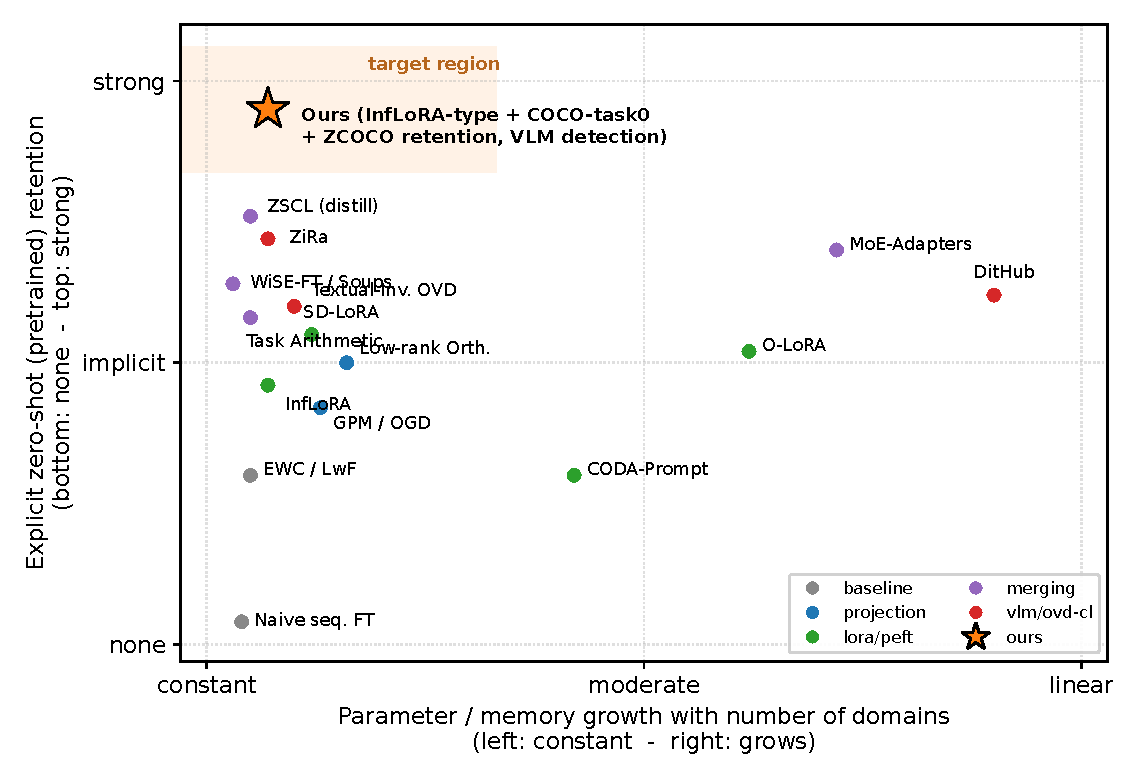
\includegraphics[width=0.9\linewidth]{figs/fig1_positioning.pdf}
\caption{既存手法の位置づけマップ．横軸はドメイン数に対するパラメータ・メモリ拡張，
縦軸は事前学習ゼロショット（ZCOCO 相当）の明示的保持機構の強さを表す．
左上の target region が本研究の狙いである．
色は手法ファミリ（baseline / projection / lora-peft / merging / vlm-ovd-cl）を示す．}
\label{fig:map}
\end{figure}

低ランクと直交部分空間という発想自体は，Chaudhry ら~\cite{lowrankorth} や InfLoRA~\cite{inflora} に
先行がある．したがって本研究の新規性は，これらを
(i) 事前学習 VLM 物体検出器（MM-Grounding DINO）上で，
(ii) COCO を task-0 として直交保護対象に含め，
(iii) ゼロショット（ZCOCO）保持を明示目標とする点に絞られる（表~\ref{tab:novelty}）．
ZiRa~\cite{zira} や DitHub~\cite{dithub} とは忘却抑制の機序が異なり（勾配部分空間の直交化 対
出力ノルム正則化・モジュール増加），パラメータ拡張一定と推論の単純さで優位を主張しうる．
また，O-LoRA~\cite{olora} がゼロショット保持を実証し，ZSCL~\cite{zscl} の特徴蒸留や
WiSE-FT~\cite{wiseft}・model soups~\cite{modelsoups}・task arithmetic~\cite{taskarith} の重み統合が
ZiRa/DitHub の外側で ZCOCO 保持の有力なベースラインかつ補完成分となる．

\begin{table}[tb]
\caption{主要手法と本研究の差別化}
\label{tab:novelty}
\small
\begin{tabularx}{\linewidth}{l c X c c c}
\hline
手法 & 設定 & 忘却抑制機序 & 拡張 & ZS保持 & 検出 \\
\hline
素朴逐次FT & 下限 & なし & 一定 & なし & --- \\
Low-rank Orth.~\cite{lowrankorth} & 分類CL & 直交部分空間（Stiefel） & 増 & 暗黙 & 否 \\
InfLoRA~\cite{inflora} & 分類CL & 勾配部分空間の直交化 & 一定 & 暗黙 & 否 \\
O-LoRA~\cite{olora} & LLM CL & 直交化損失 & 線形増 & 実証 & 否 \\
ZiRa~\cite{zira} & VLM検出 & 出力ノルム正則化（ZiL） & 一定 & 明示 & 是 \\
DitHub~\cite{dithub} & VLM検出 & モジュール分離・統合 & 増 & 明示 & 是 \\
本研究 & VLM検出 & 勾配直交化＋COCO保護 & 一定 & 明示 & 是 \\
\hline
\end{tabularx}
\end{table}

%==================================================================
\section{まとめと今後の課題}
\label{sec:conclusion}
広域な既存研究の調査により，本研究は次の三点で位置づけられる．
第一に，本設定は形式的に DIL（クラス非重複のハイブリッド）であり忘却は原理的に困難で，
NTK 理論・勾配部分空間・内在次元・線形モード接続性が，提案手法の理論的支柱であると同時に
機序分析の道具を与える（第\ref{sec:theory}・\ref{sec:toolbox}節）．
第二に，ZCOCO 保持は適応・過去ドメイン忘却とは独立した故障モードであり，
特徴蒸留・重み統合・推論時ルーティングが ZiRa/DitHub の外側で必須のベースライン群となる
（第\ref{sec:vlmcl}節）．
第三に，評価は Roboflow100-VL を軸に，OVD 適応・MoE の近年研究も比較に含めるべきである
（第\ref{sec:ovd}節）．

今後検証すべき主要な問いは次の通りである．
(1) 重み統合・特徴蒸留・ルーティングは grounded detector で成立するか
（既存実証の多くは CLIP 分類である）．
(2) NTK・GPM 流のアラインメント測定は大規模検出器・非重複ラベルで忘却を予測できるか．
(3)「忘却は分類側に局在し回帰側は頑健」という二段検出器の知見は，
MM-Grounding DINO のクエリ・対照ヘッドへ転移するか．
(4) 直交化 LoRA と COCO 保護，および各補完成分（蒸留・統合・ルーティング）は
加算的か，冗長か，競合か，そして最良の適応・保持・ZCOCO のパレート前線はどれか．

\bibliographystyle{splncs04}
\bibliography{ref}

\end{document}
